\documentclass[10pt]{beamer}
\usepackage[english]{babel}
\usepackage[utf8]{inputenc}
\usepackage[T1]{fontenc}
\usepackage{helvet}
\usepackage{listings}
\usepackage{multicol}
\usepackage{cite}

%-------------------------------------------------------
% INFORMATION IN THE TITLE PAGE
%-------------------------------------------------------

\newcommand{\cstitle}{\textbf{Bioinformatics}}
\subtitle[]{An analysis of alignment-free methods using image textures from DNA sequences}
\newcommand{\cscourseCode}{1005155}
\newcommand{\csauthor}{MSc. Vicente Machaca Arceda}
\institute[UNSA]{Universidad Nacional de San Agustín de Arequipa}
\newcommand{\csemail}{vmachacaa@unsa.edu.pe}
\newcommand{\instituteabr}{UNSA}
\newcommand{\nameUp}{ICC Fase 1}
\date{\today}
\title[\cscourseCode]{\cstitle}
\author{\csauthor}
%%%%%%%%%%%%%%%%%

%-------------------------------------------------------
% INFORMATION IN THE TITLE PAGE
%-------------------------------------------------------

%-------------------------------------------------------
% SOLUTION
%-------------------------------------------------------
\def\mysol{0} 
\def\mysol{1} 
%-------------------------------------------------------


%-------------------------------------------------------
% CHOOSE THE THEME
%-------------------------------------------------------
\def\mycmd{0} % CS THEME
%\def\mycmd{1} % MYTHEME
%-------------------------------------------------------


\if\mycmd1
\usetheme[]{Feather}
\newcommand{\chref}[2]{	\href{#1}{{\usebeamercolor[bg]{Feather}#2}} }
\else
\usepackage{csformat}
\fi

\newcommand{\1}{
	\setbeamertemplate{background}{
		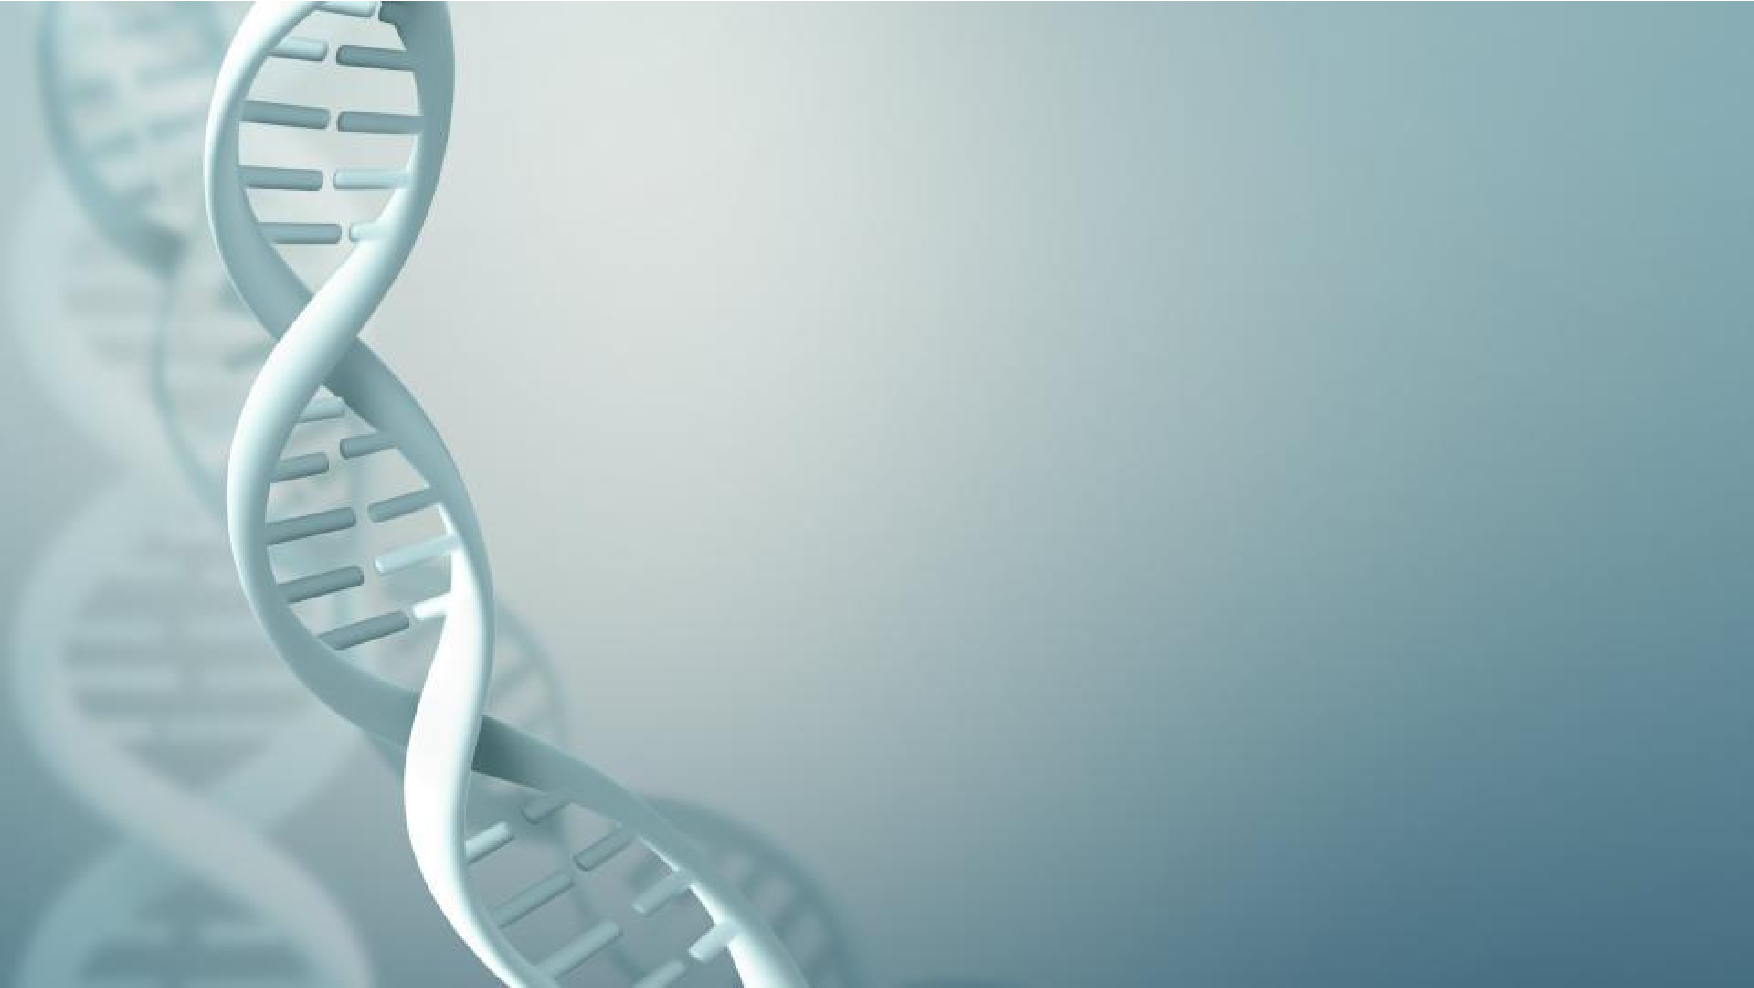
\includegraphics[width=\paperwidth,height=\paperheight]{img/1}
		\tikz[overlay] \fill[fill opacity=0.75,fill=white] (0,0) rectangle (-\paperwidth,\paperheight);
	}
}



%-------------------------------------------------------
% THE BODY OF THE PRESENTATION
%-------------------------------------------------------

\begin{document}
	
	
	\AtBeginSubsection[]
	{
		\begin{frame}
			\frametitle{Table of Contents}
			\tableofcontents[currentsubsection]
		\end{frame}
	}
	
	
	%-------------------------------------------------------
	% THE TITLEPAGE
	%-------------------------------------------------------
	
	\if\mycmd1 % MY THEME
	\1{
		\begin{frame}[plain,noframenumbering] 
			\titlepage 
	\end{frame}}
	\else % CS THEME
	\maketitle
	\fi
	
	%-------------------------------------------------------
	%-------------------------------------------------------
	\begin{frame}{Table of Contents}
		\tableofcontents
	\end{frame}
	%-------------------------------------------------------
	%-------------------------------------------------------


%%%%%%%%%%%%%%%%%%%%%%%%%%%%%%%%%%%%%%%%%%%%%%%%%%%%%%%%%%%%%%%%%%%%%%%%%%%%%%%%%%%%%%%%%%%%%%%%%%%%%%%%%%%%%%%%
%%%%%%%%%%%%%%%%%%%%%%%%%%%%%%%%%%%%%%%%%%%%%%%%%%%%%%%%%%%%%%%%%%%%%%%%%%%%%%%%%%%%%%%%%%%%%%%%%%%%%%%%%%%%%%%%
\section{Introduction}
%%%%%%%%%%%%%%%%%%%%%%%%%%%%%%%%%%%%%%%%%%%%%%%%%%%%%%%%%%%%%%%%%%%%%%%%%%%%%%%%%%%%%%%%%%%%%%%%%%%%%%%%%%%%%%%%
%%%%%%%%%%%%%%%%%%%%%%%%%%%%%%%%%%%%%%%%%%%%%%%%%%%%%%%%%%%%%%%%%%%%%%%%%%%%%%%%%%%%%%%%%%%%%%%%%%%%%%%%%%%%%%%%

%-------------------------------------------------------
%-------------------------------------------------------
%\begin{frame}{Introduction}{DNA}
%\begin{figure}[]
%	\centering
%	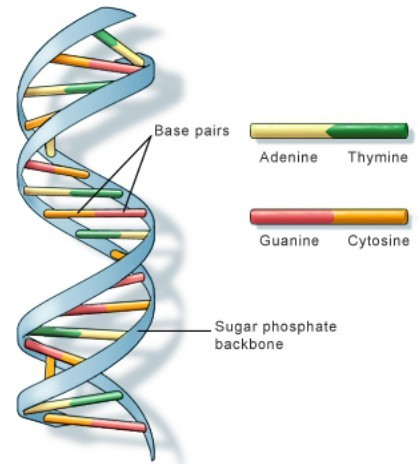
\includegraphics[width=0.5\textwidth,keepaspectratio]{img/mineria/bio6}
%	%\label{img:mot2}
%	\caption{Molecules in DNA. Adenine, Thymine, Guanine and Cytosine \cite{dna2020located}.}
%\end{figure}
%\end{frame}
%-------------------------------------------------------
%-------------------------------------------------------

%-------------------------------------------------------
%-------------------------------------------------------
\begin{frame}{Introduction}{DNA sequence}
	\begin{figure}[]
		\centering
		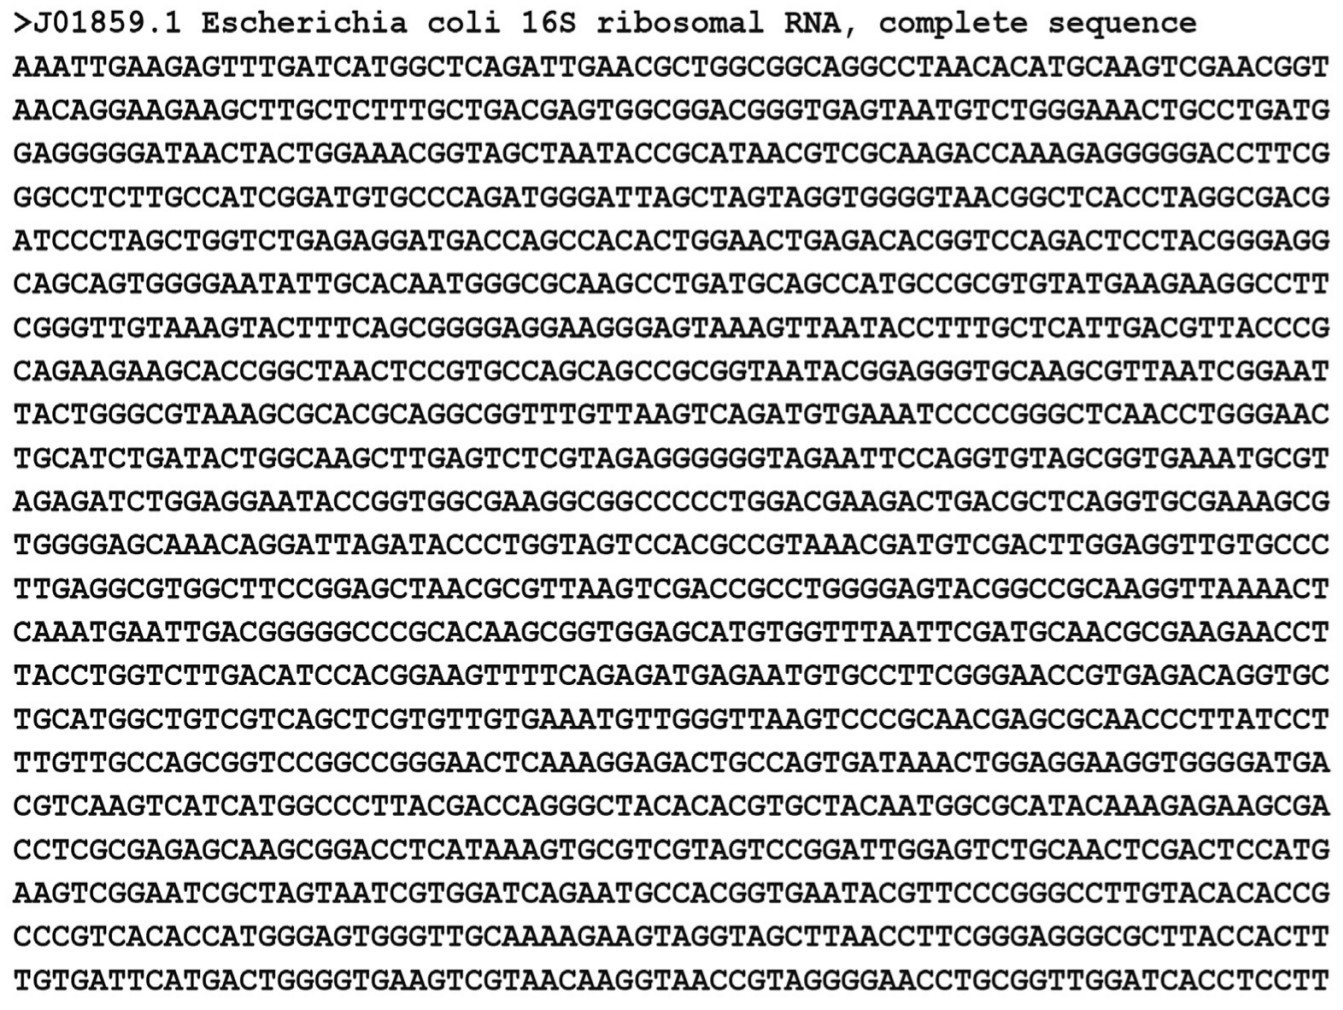
\includegraphics[width=\textwidth,height=0.7\textheight,keepaspectratio]{img/mineria/dnaimg_1}
		\label{img:mot2}
		\caption{16S ribosomal DNA of Escherichia coli with FASTA Format.}
	\end{figure}
\end{frame}
%-------------------------------------------------------
%-------------------------------------------------------

%-------------------------------------------------------
%-------------------------------------------------------
\begin{frame}{Introduction}{DNA sequence}%
	\begin{block}{}
		\centering
		The human genome is made of \textbf{\string ~3.2 billions bp} of DNA. \\
		\string ~6.4 billions of nucleotides \cite{archibald2018genomics}.
	\end{block}
	
	\begin{block}{}
		\centering
		The HIV-1 genome is made of \textbf{\string ~20k bp} of DNA. \\
		Meanwhile, the COVID-19 is made of \textbf{\string ~32k bp} \cite{randhawa2020machine}.
	\end{block}	
\end{frame}
%-------------------------------------------------------
%-------------------------------------------------------

%-------------------------------------------------------
%-------------------------------------------------------
%\begin{frame}{Introduction}{DNA}
%\begin{table}[]
%	\caption{Total GigaBytes used to store a complete diploid genome.}
%	\begin{tabular}{ll}
%		\hline
%		DNA bases                & 4           \\
%		Bits per base            & 2           \\
%		Base pairs per genome    & 3200000000  \\
%		Bits per genome          & 12800000000 \\
%		Total bits Diplod genome & 25600000000 \\
%		Total Kilobytes          & 3125000     \\
%		Total Megabytes          & 3052        \\
%		\hline
%		\textbf{Total Gigabytes}          & \textbf{2.980}      \\
%		\hline
%	\end{tabular}
%\end{table}
%\end{frame}
%-------------------------------------------------------
%-------------------------------------------------------

%-------------------------------------------------------
%-------------------------------------------------------
%\begin{frame}{Introduction}{DNA}
%	\begin{figure}[]
%		\centering
%		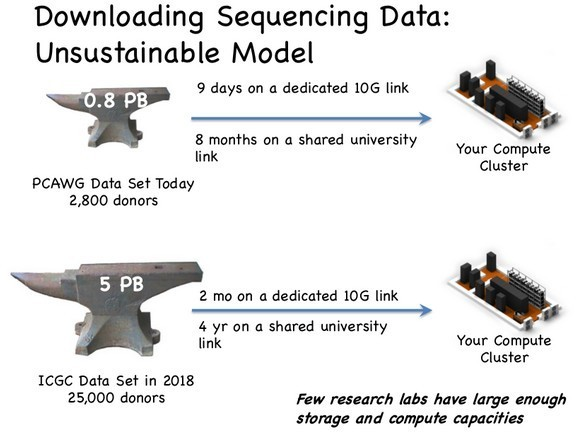
\includegraphics[width=\textwidth,height=0.7\textheight,keepaspectratio]{img/mineria/dat.jpg}
%		\label{img:mot2}
%		\caption{Downloading sequencing data}
%	\end{figure}
%\end{frame}
%-------------------------------------------------------
%-------------------------------------------------------


%-------------------------------------------------------
%-------------------------------------------------------
%\begin{frame}{Introduction}{Similarity and Phylogenetics}
%	\begin{block}{Similarity}
%		It is used for identifying evolutionary or affinity relations \cite{delibacs2020dna}. Similarity analysis is an important r%esearch area in Bioinformatics \cite{jin2017similarity}.
%	\end{block}
	
%	\begin{block}{Phylogenetics}
%		Phylogenetics is the study of the evolutionary history of living organisms using tree-
%		like diagrams to represent pedigrees of these organisms \cite{xiong2006essential}.
%	\end{block}
%\end{frame}
%-------------------------------------------------------
%-------------------------------------------------------

%-------------------------------------------------------
%-------------------------------------------------------
%\begin{frame}{Introduction}{}
%	\begin{figure}[]
%		\centering
%		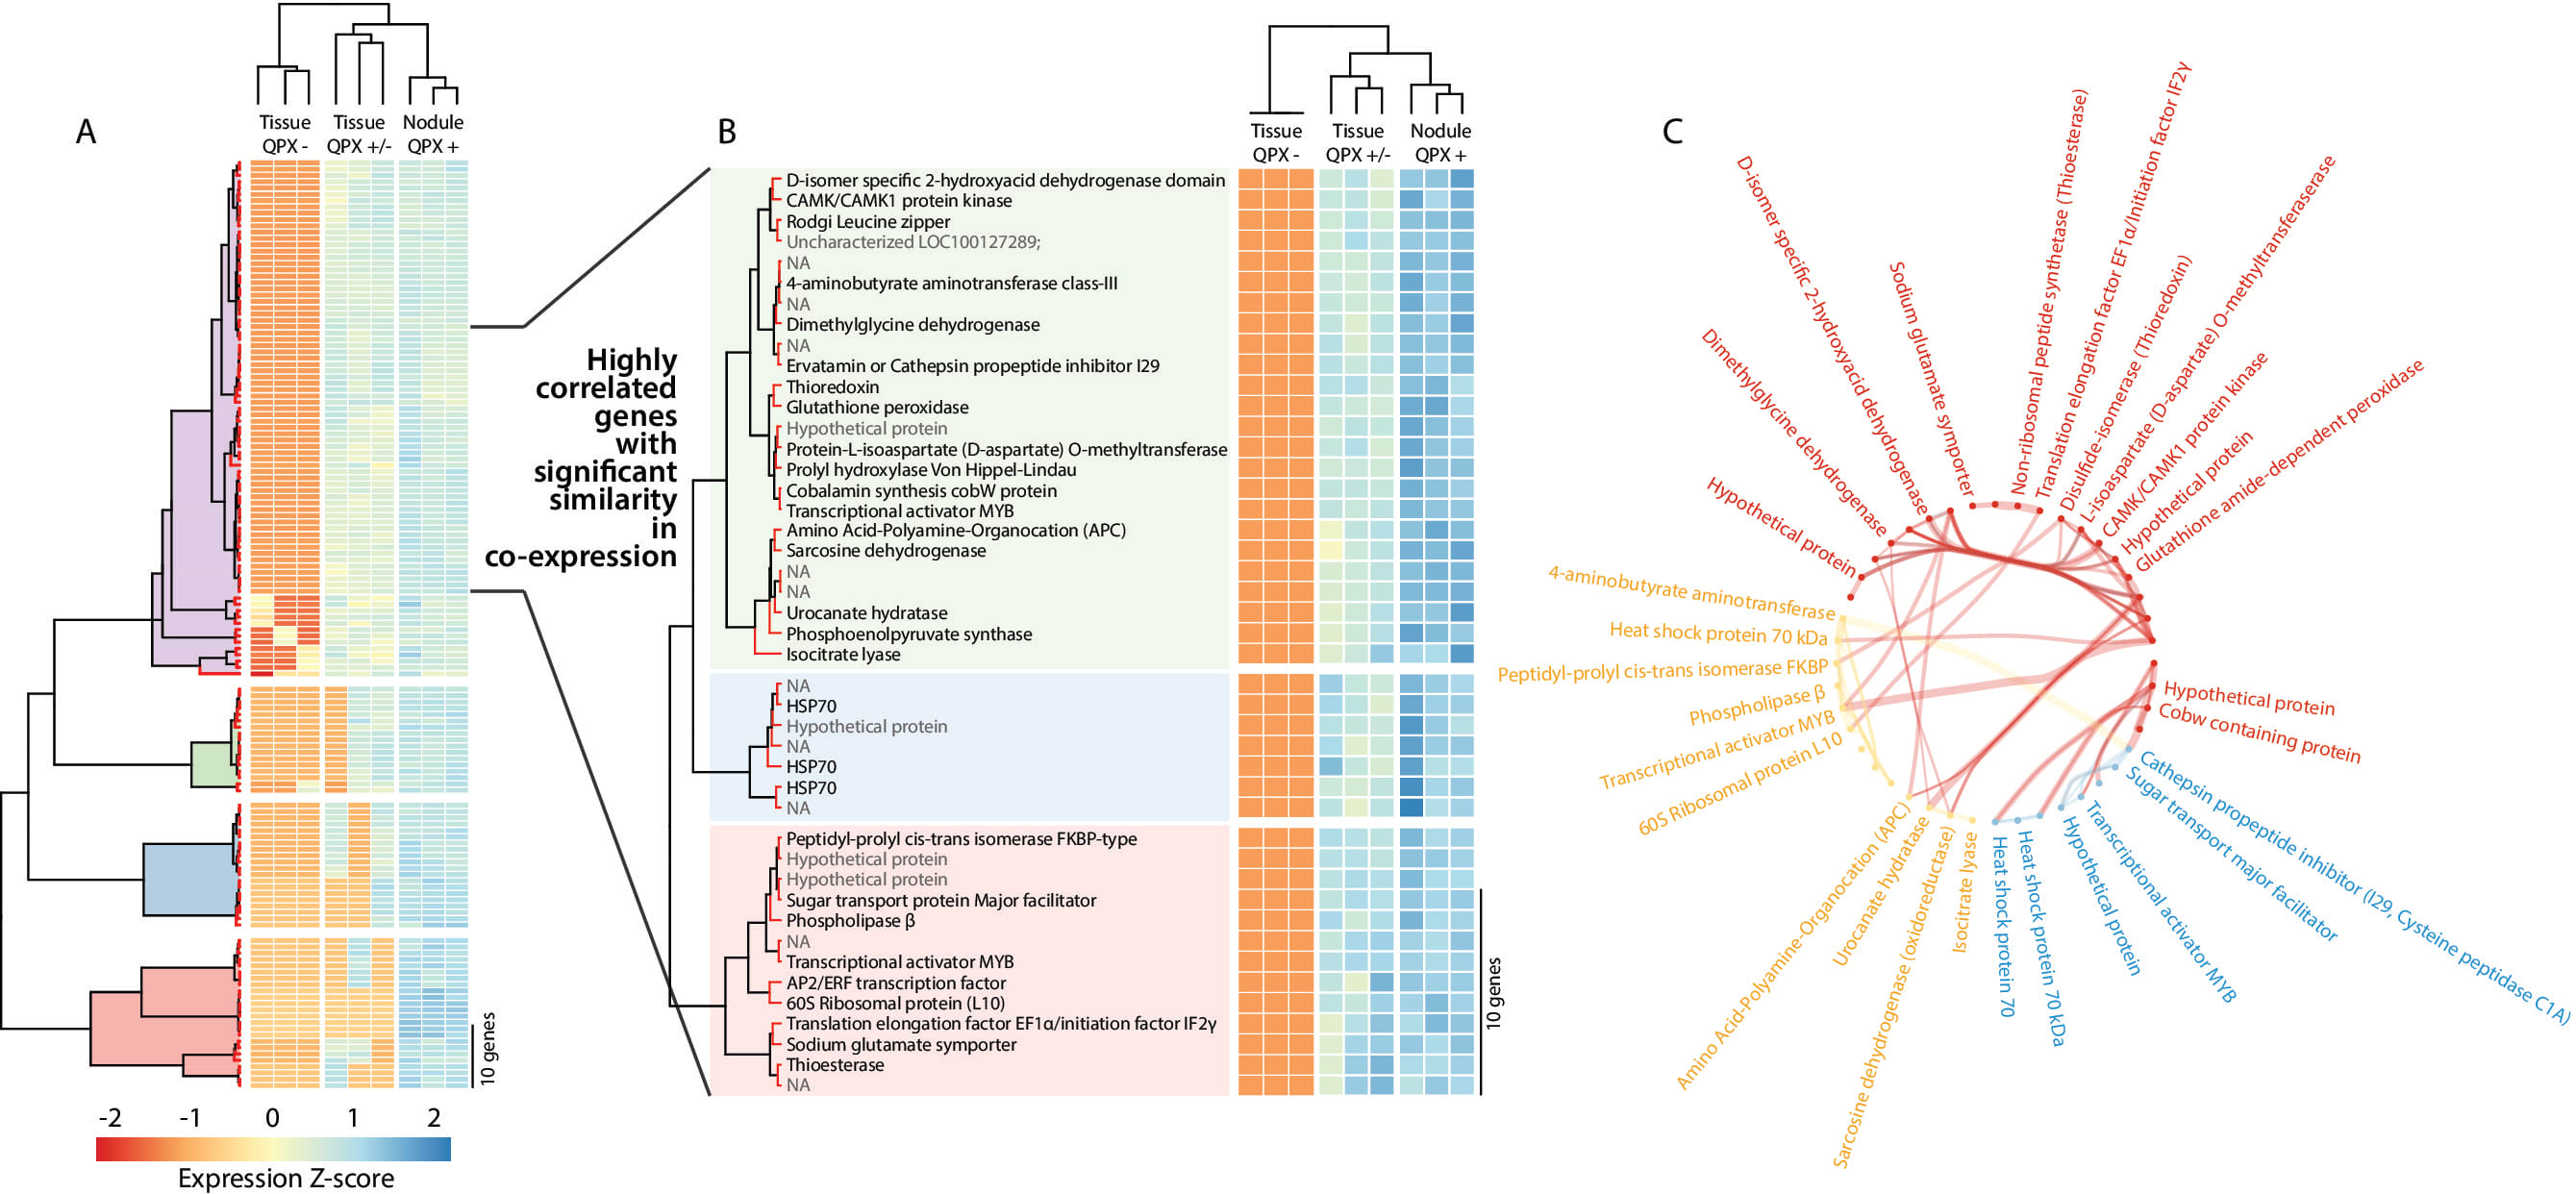
\includegraphics[width=\textwidth,keepaspectratio]{img/mineria/dna_visualization.jpg}
%		\label{img:mot2}
%		\caption{Example of visualization in bioinformatics.}
%	\end{figure}
%\end{frame}
%-------------------------------------------------------
%-------------------------------------------------------


%%%%%%%%%%%%%%%%%%%%%%%%%%%%%%%%%%%%%%%%%%%%%%%%%%%%%%%%%%%%%%%%%%%%%%%%%%%%%%%%%%%%%%%%%%%%%%%%%%%%%%%%%%%%%%%%
%%%%%%%%%%%%%%%%%%%%%%%%%%%%%%%%%%%%%%%%%%%%%%%%%%%%%%%%%%%%%%%%%%%%%%%%%%%%%%%%%%%%%%%%%%%%%%%%%%%%%%%%%%%%%%%%
%\subsection{Similarity and Phylogenetics}
%%%%%%%%%%%%%%%%%%%%%%%%%%%%%%%%%%%%%%%%%%%%%%%%%%%%%%%%%%%%%%%%%%%%%%%%%%%%%%%%%%%%%%%%%%%%%%%%%%%%%%%%%%%%%%%%
%%%%%%%%%%%%%%%%%%%%%%%%%%%%%%%%%%%%%%%%%%%%%%%%%%%%%%%%%%%%%%%%%%%%%%%%%%%%%%%%%%%%%%%%%%%%%%%%%%%%%%%%%%%%%%%%



%%%%%%%%%%%%%%%%%%%%%%%%%%%%%%%%%%%%%%%%%%%%%%%%%%%%%%%%%%%%%%%%%%%%%%%%%%%%%%%%%%%%%%%%%%%%%%%%%%%%%%%%%%%%%%%%
%%%%%%%%%%%%%%%%%%%%%%%%%%%%%%%%%%%%%%%%%%%%%%%%%%%%%%%%%%%%%%%%%%%%%%%%%%%%%%%%%%%%%%%%%%%%%%%%%%%%%%%%%%%%%%%%
%\subsection{Motivation}
%%%%%%%%%%%%%%%%%%%%%%%%%%%%%%%%%%%%%%%%%%%%%%%%%%%%%%%%%%%%%%%%%%%%%%%%%%%%%%%%%%%%%%%%%%%%%%%%%%%%%%%%%%%%%%%%
%%%%%%%%%%%%%%%%%%%%%%%%%%%%%%%%%%%%%%%%%%%%%%%%%%%%%%%%%%%%%%%%%%%%%%%%%%%%%%%%%%%%%%%%%%%%%%%%%%%%%%%%%%%%%%%%

%-------------------------------------------------------
%-------------------------------------------------------
%\begin{frame}{Introduction}{Motivation}
%	\begin{itemize}
%		\item \textbf{Knowledge domain:} Bioinformatics.
%		\item \textbf{Users:} Biologists and bioinformaticians.
%		\item \textbf{Why?:} It could be the beginning of a new set of similarity algorithms in Bioinfomratics.
%		\item \textbf{Questions}: The alignment-free methods using images textures from DNA could replace classics algorithms as BLAST and CLUSTALW.
%	\end{itemize}
%\end{frame}
%-------------------------------------------------------
%-------------------------------------------------------


%-------------------------------------------------------
%-------------------------------------------------------
%\begin{frame}{Introduction}{Phylogenetics}
%	\begin{figure}[]
%		\centering
%		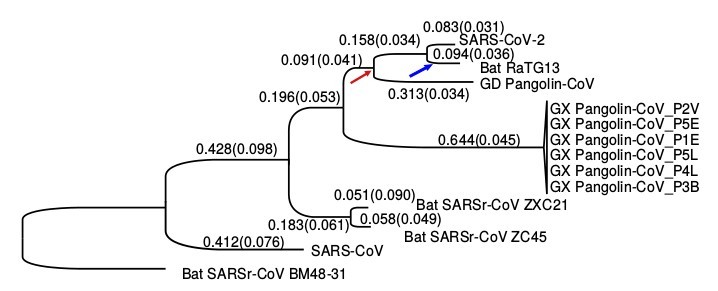
\includegraphics[width=\textwidth,height=0.7\textheight,keepaspectratio]{img/mineria/phylocovid.jpg}
%		\label{img:mot2}
%		\caption{The phylogenetic tree of SARS-CoV-2 (COVID-19) and the related Coronaviruses  \cite{tang2020origin}.}
%	\end{figure}
%\end{frame}
%-------------------------------------------------------
%-------------------------------------------------------

%-------------------------------------------------------
%-------------------------------------------------------
%\begin{frame}{Introduction}{Phylogenetics}
%	\begin{figure}[]
%		\centering
%		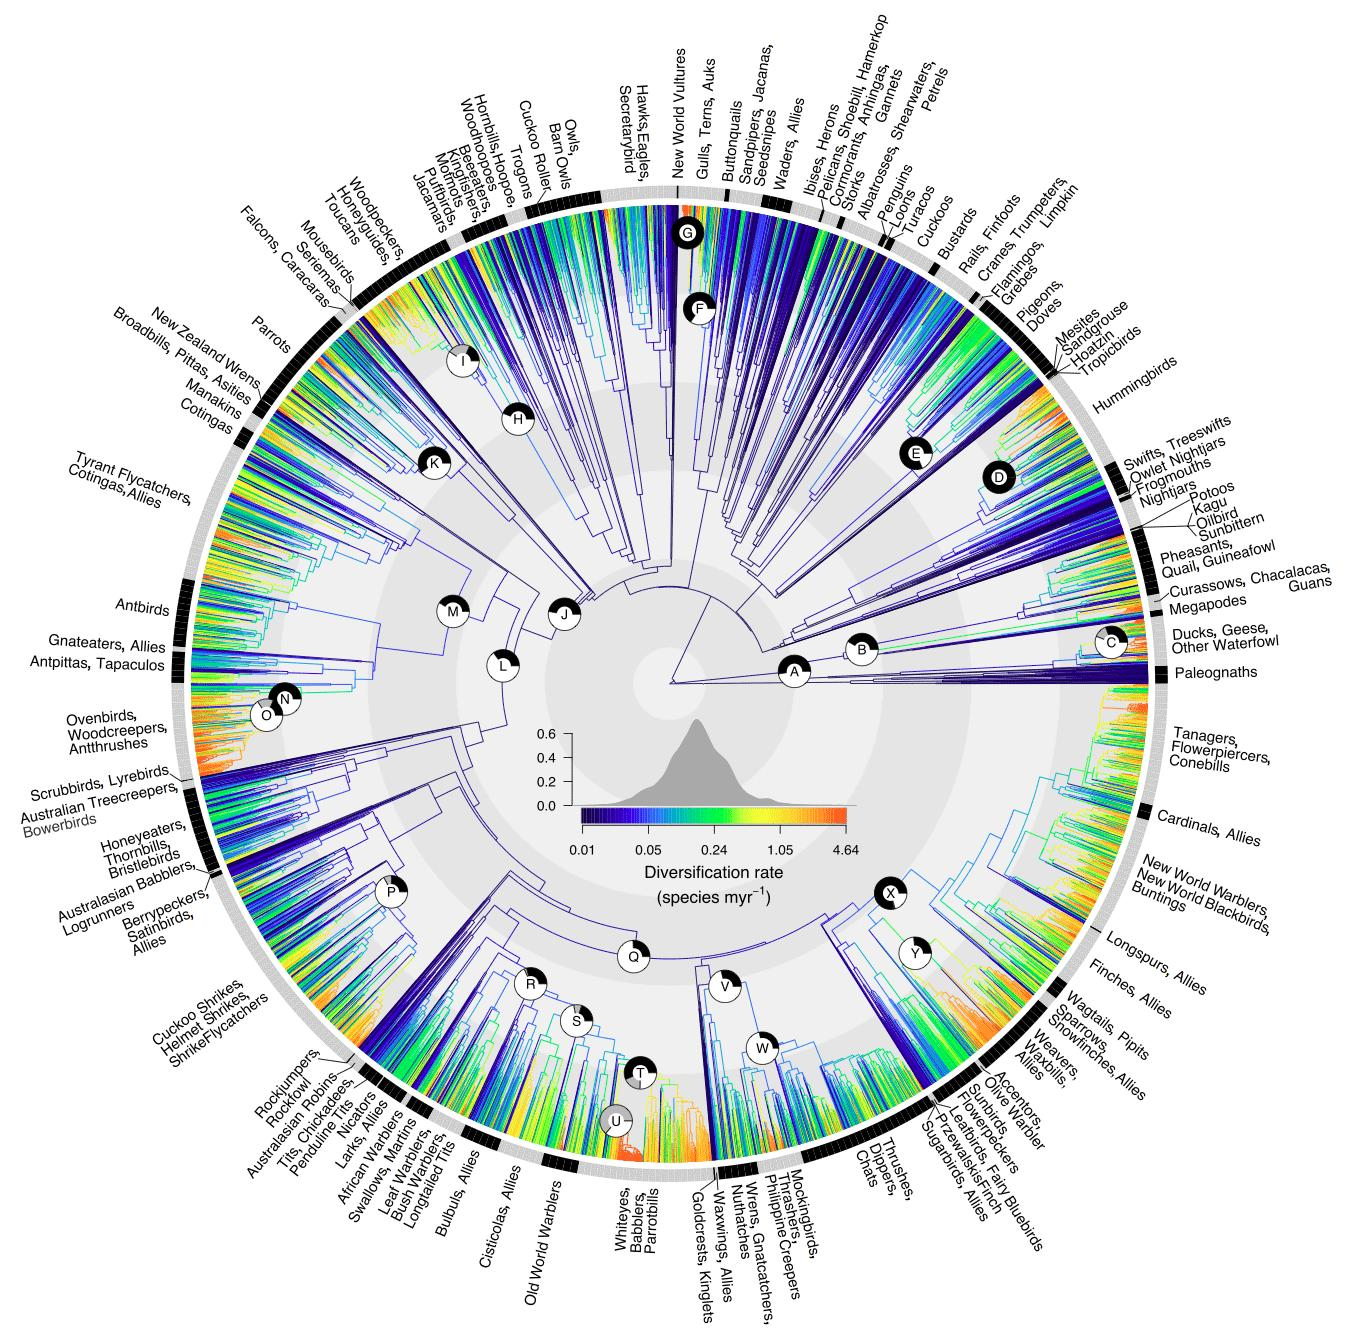
\includegraphics[width=\textwidth,height=0.7\textheight,keepaspectratio]{img/mineria/phylo.jpg}
%		\label{img:mot2}
%		\caption{The phylogeny tree of bird species  \cite{phylobirds2020}.}
%	\end{figure}
%\end{frame}
%-------------------------------------------------------
%-------------------------------------------------------





%%%%%%%%%%%%%%%%%%%%%%%%%%%%%%%%%%%%%%%%%%%%%%%%%%%%%%%%%%%%%%%%%%%%%%%%%%%%%%%%%%%%%%%%%%%%%%%%%%%%%%%%%%%%%%%%
%%%%%%%%%%%%%%%%%%%%%%%%%%%%%%%%%%%%%%%%%%%%%%%%%%%%%%%%%%%%%%%%%%%%%%%%%%%%%%%%%%%%%%%%%%%%%%%%%%%%%%%%%%%%%%%%
\subsection{Problem}
%%%%%%%%%%%%%%%%%%%%%%%%%%%%%%%%%%%%%%%%%%%%%%%%%%%%%%%%%%%%%%%%%%%%%%%%%%%%%%%%%%%%%%%%%%%%%%%%%%%%%%%%%%%%%%%%
%%%%%%%%%%%%%%%%%%%%%%%%%%%%%%%%%%%%%%%%%%%%%%%%%%%%%%%%%%%%%%%%%%%%%%%%%%%%%%%%%%%%%%%%%%%%%%%%%%%%%%%%%%%%%%%%

%-------------------------------------------------------
%-------------------------------------------------------
\begin{frame}{Problem}{Phylogenetics steps}
	\begin{figure}[]
		\centering
		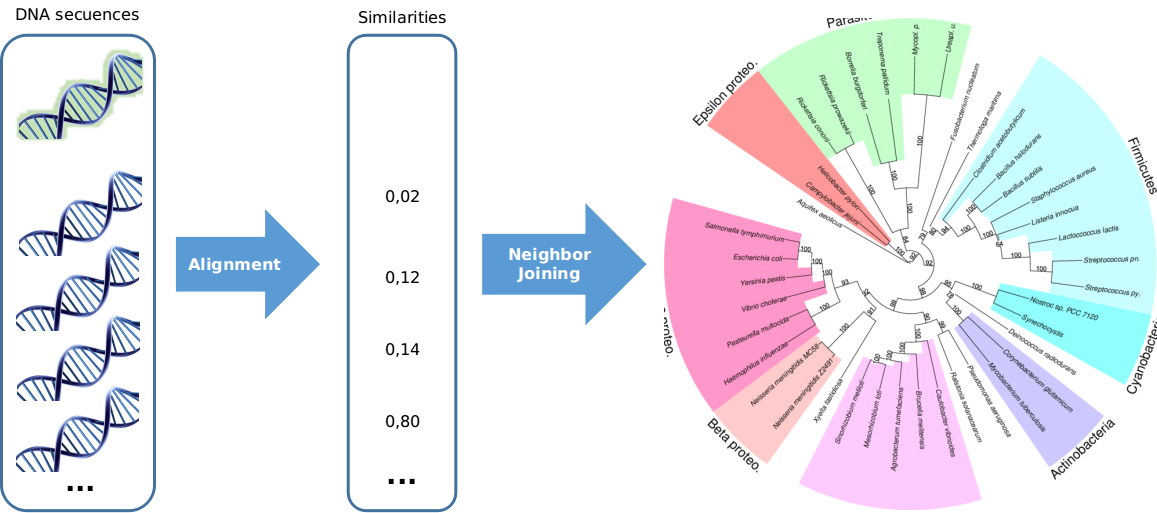
\includegraphics[width=\textwidth,height=0.7\textheight,keepaspectratio]{img/mineria/phylo2}
		\label{img:mot2}
		\caption{Steps to visualize phylonetics trees.}
	\end{figure}
\end{frame}
%-------------------------------------------------------
%-------------------------------------------------------

%-------------------------------------------------------
%-------------------------------------------------------
\begin{frame}{Problem}{Phylogenetics steps}
	\begin{figure}[]
		\centering
		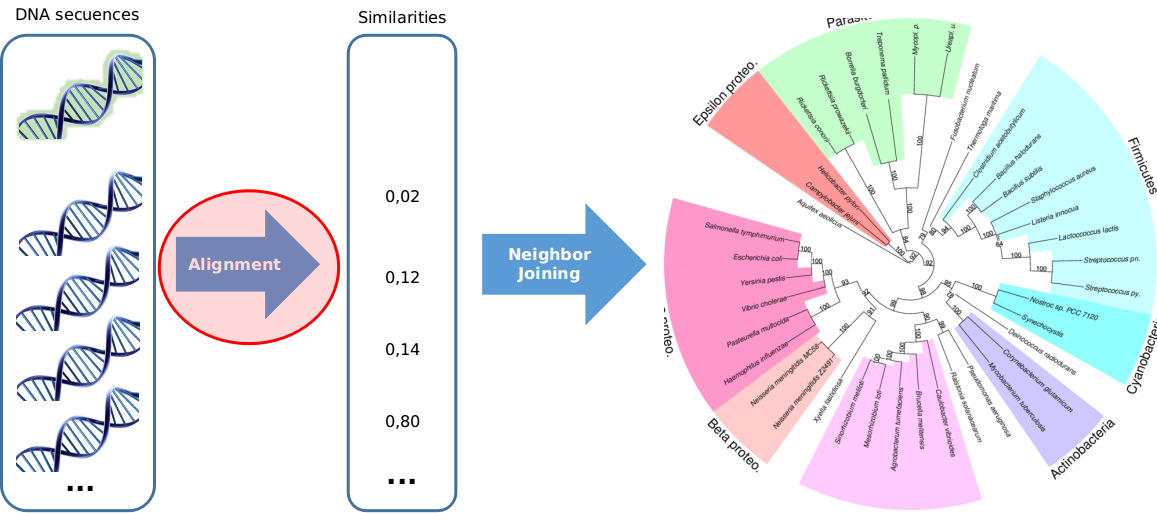
\includegraphics[width=\textwidth,height=0.7\textheight,keepaspectratio]{img/mineria/phylo3}
		\label{img:mot2}
		\caption{Steps to visualize phylonetics trees.}
	\end{figure}
\end{frame}
%-------------------------------------------------------
%-------------------------------------------------------


%-------------------------------------------------------
%-------------------------------------------------------
\begin{frame}{Problem}{Alignment-based methods}
	\begin{block}{}
		\begin{itemize}
			\item The most used \textbf{alignment-based} method are BLAST and CLUSTALW. \pause
			\item They are slow. For example, it take one hour to align 18 sequences of 18k bp. \pause
			\item DNA sequences increases every day so \textbf{alignment-based} methods get slower every second. \pause		 	
			%\item For example, two days were necessary to build the Phylogenetis tree of COVID-19. 
		\end{itemize}
	\end{block}
\end{frame}
%-------------------------------------------------------
%-------------------------------------------------------

%%%%%%%%%%%%%%%%%%%%%%%%%%%%%%%%%%%%%%%%%%%%%%%%%%%%%%%%%%%%%%%%%%%%%%%%%%%%%%%%%%%%%%%%%%%%%%%%%%%%%%%%%%%%%%%%
%%%%%%%%%%%%%%%%%%%%%%%%%%%%%%%%%%%%%%%%%%%%%%%%%%%%%%%%%%%%%%%%%%%%%%%%%%%%%%%%%%%%%%%%%%%%%%%%%%%%%%%%%%%%%%%%
\subsection{Objective}
%%%%%%%%%%%%%%%%%%%%%%%%%%%%%%%%%%%%%%%%%%%%%%%%%%%%%%%%%%%%%%%%%%%%%%%%%%%%%%%%%%%%%%%%%%%%%%%%%%%%%%%%%%%%%%%%
%%%%%%%%%%%%%%%%%%%%%%%%%%%%%%%%%%%%%%%%%%%%%%%%%%%%%%%%%%%%%%%%%%%%%%%%%%%%%%%%%%%%%%%%%%%%%%%%%%%%%%%%%%%%%%%%

%-------------------------------------------------------
%-------------------------------------------------------
\begin{frame}{Objective}{}
	\begin{block}{}
		Compare  \textbf{alignment-free} algorithms based on texture descriptors, against CLUSTALW. 
		\begin{itemize}
			\item First-Order Statistics  \textbf{(FOS)} \cite{delibacs2020dna}.
			\item Gray Level Co-ocurrence Matrix \textbf{(GLCM)} \cite{chen2018use}.
			\item Multi-resolution Local Binary Patterns \textbf{(MLBP)} \cite{kouchaki2019signal}.
		\end{itemize}
	\end{block}

\end{frame}
%-------------------------------------------------------
%-------------------------------------------------------

%-------------------------------------------------------
%-------------------------------------------------------
%\begin{frame}{Proposal}{Pipeline}
%	\begin{figure}[]
%		\centering
%		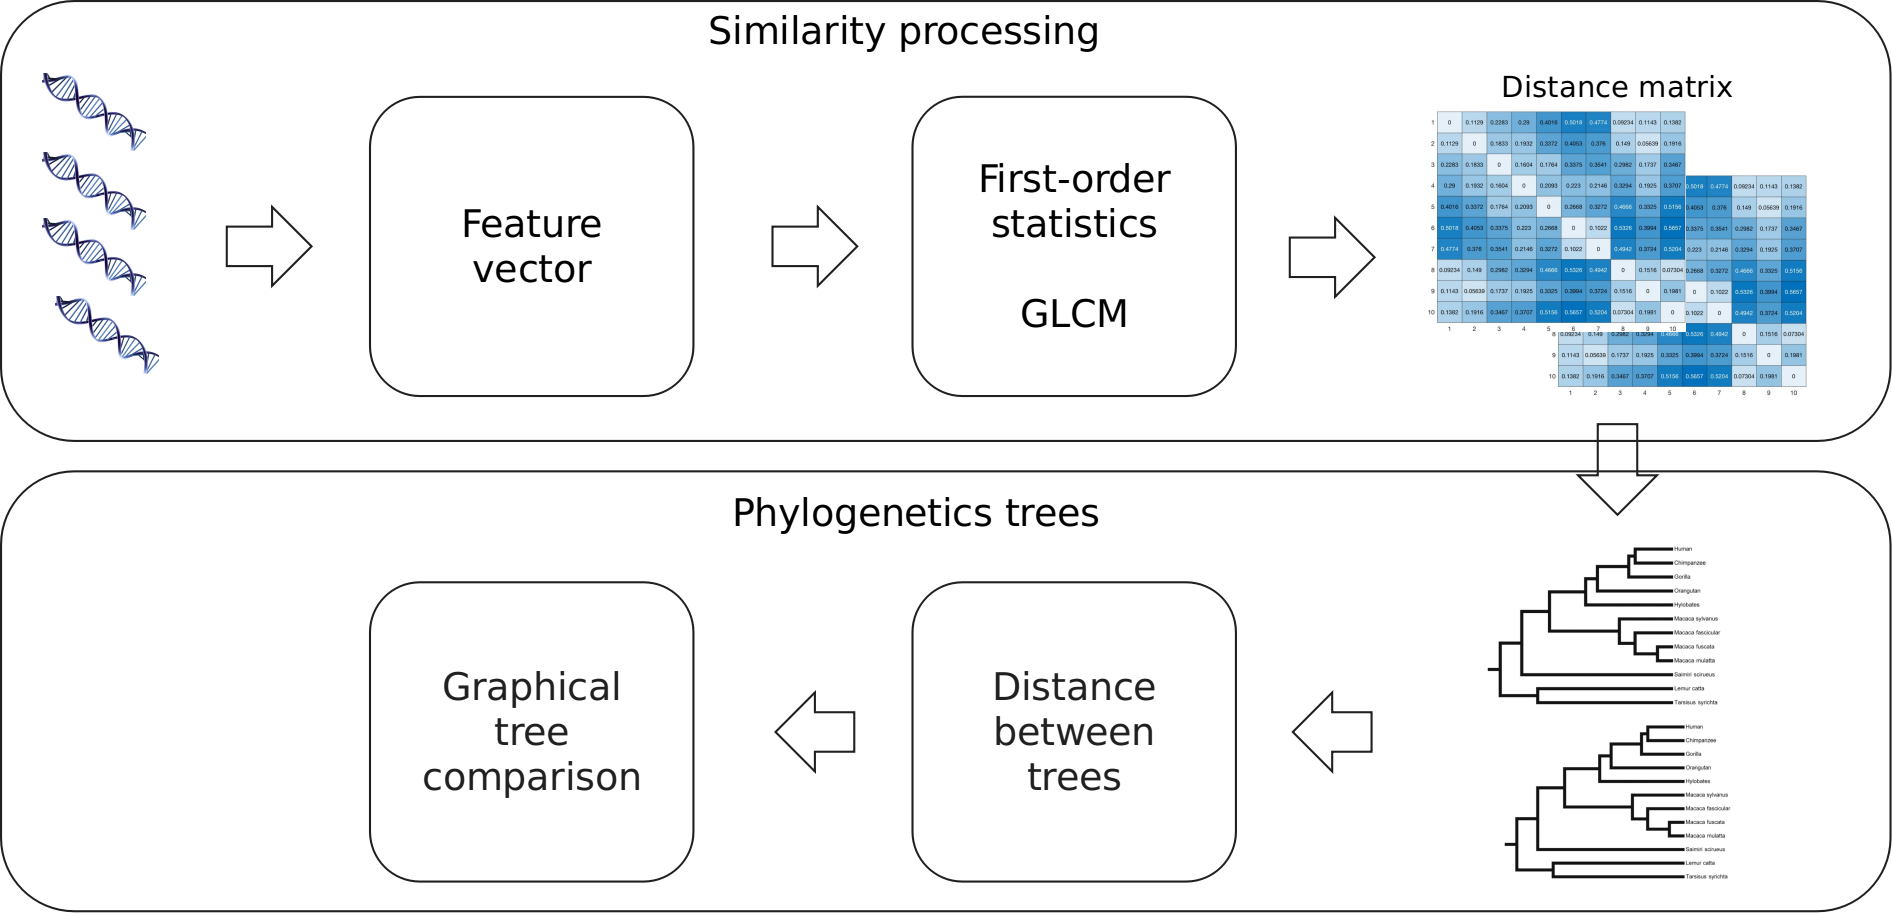
\includegraphics[width=\textwidth,height=0.7\textheight,keepaspectratio]{img/mineria/pipeline}
%		%\label{img:mot2}
		%\caption{16S ribosomal DNA of Escherichia coli with FASTA Format.}
%	\end{figure}
%\end{frame}
%-------------------------------------------------------
%-------------------------------------------------------

%%%%%%%%%%%%%%%%%%%%%%%%%%%%%%%%%%%%%%%%%%%%%%%%%%%%%%%%%%%%%%%%%%%%%%%%%%%%%%%%%%%%%%%%%%%%%%%%%%%%%%%%%%%%%%%%
%%%%%%%%%%%%%%%%%%%%%%%%%%%%%%%%%%%%%%%%%%%%%%%%%%%%%%%%%%%%%%%%%%%%%%%%%%%%%%%%%%%%%%%%%%%%%%%%%%%%%%%%%%%%%%%%
\section{Alignment-free methods base on image textures}
%%%%%%%%%%%%%%%%%%%%%%%%%%%%%%%%%%%%%%%%%%%%%%%%%%%%%%%%%%%%%%%%%%%%%%%%%%%%%%%%%%%%%%%%%%%%%%%%%%%%%%%%%%%%%%%%
%%%%%%%%%%%%%%%%%%%%%%%%%%%%%%%%%%%%%%%%%%%%%%%%%%%%%%%%%%%%%%%%%%%%%%%%%%%%%%%%%%%%%%%%%%%%%%%%%%%%%%%%%%%%%%%%

%%%%%%%%%%%%%%%%%%%%%%%%%%%%%%%%%%%%%%%%%%%%%%%%%%%%%%%%%%%%%%%%%%%%%%%%%%%%%%%%%%%%%%%%%%%%%%%%%%%%%%%%%%%%%%%%
%%%%%%%%%%%%%%%%%%%%%%%%%%%%%%%%%%%%%%%%%%%%%%%%%%%%%%%%%%%%%%%%%%%%%%%%%%%%%%%%%%%%%%%%%%%%%%%%%%%%%%%%%%%%%%%%
\subsection{First-order statistics (FOS)} \label{section:fos}
%%%%%%%%%%%%%%%%%%%%%%%%%%%%%%%%%%%%%%%%%%%%%%%%%%%%%%%%%%%%%%%%%%%%%%%%%%%%%%%%%%%%%%%%%%%%%%%%%%%%%%%%%%%%%%%%
%%%%%%%%%%%%%%%%%%%%%%%%%%%%%%%%%%%%%%%%%%%%%%%%%%%%%%%%%%%%%%%%%%%%%%%%%%%%%%%%%%%%%%%%%%%%%%%%%%%%%%%%%%%%%%%%

%-------------------------------------------------------
%-------------------------------------------------------
%\begin{frame}{FOS}{Method 1}
%	\begin{block}{DNA sequence similarity analysis using image texture analysis based	on first-order statistics}
%		The authors used \textbf{alignment-free} methods that convert the DNA sequences into feature vectors. They represent DNA sequences as images and then computed the histogram \cite{delibacs2020dna}. 
%	\end{block}
%\end{frame}
%-------------------------------------------------------
%-------------------------------------------------------

%-------------------------------------------------------
%-------------------------------------------------------
%\begin{frame}{FOS}{Method 1}%
%	\begin{figure}[]
%		\centering
%		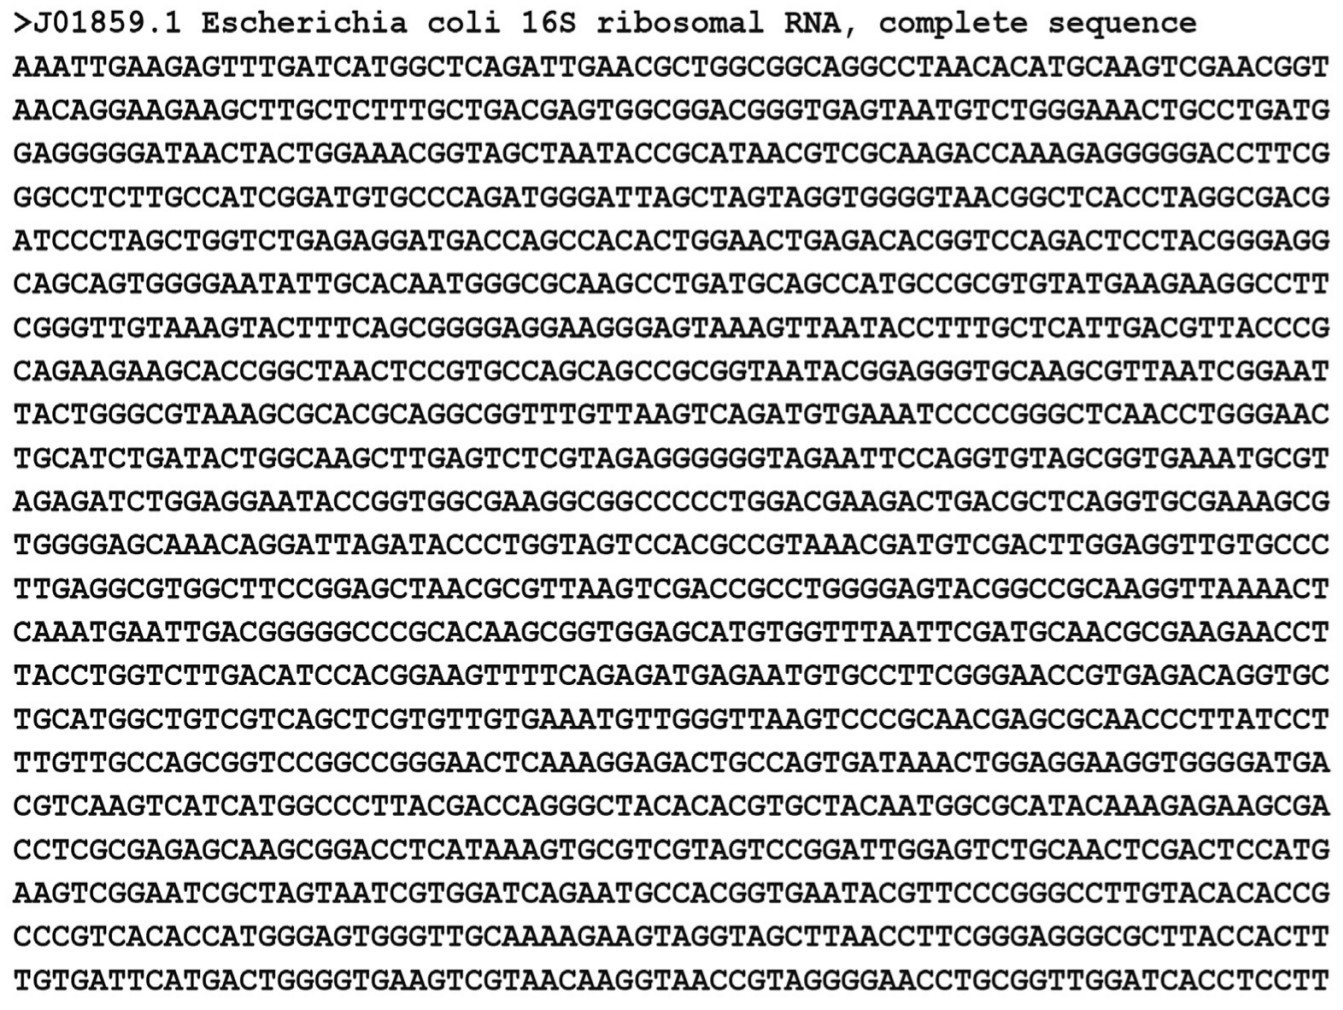
\includegraphics[width=\textwidth,height=0.7\textheight,keepaspectratio]{img/mineria/dnaimg_1}
%		\label{img:mot2}
%		\caption{16S ribosomal DNA of Escherichia coli with FASTA Format.}
%	\end{figure}
%\end{frame}
%-------------------------------------------------------
%-------------------------------------------------------

%-------------------------------------------------------
%-------------------------------------------------------
\begin{frame}{FOS}{Mapping function }
	\begin{block}{}
		Each pair of bases have a value from $0$ to $15$.
		
		\begin{equation}
		\alpha = \left\lbrace \begin{tabular}{l}
		$AA, AG, AC, AT, GA, GG, GC, GT,$\\
		$CG, CC, CT, CA, TA, TG, TC, TT$
		\end{tabular}      
		\right\rbrace
		\end{equation}
		
	\end{block}
\end{frame}
%-------------------------------------------------------
%-------------------------------------------------------


%-------------------------------------------------------
%-------------------------------------------------------
\begin{frame}{FOS}{Image from DNA}
	\begin{figure}[]
		\centering
		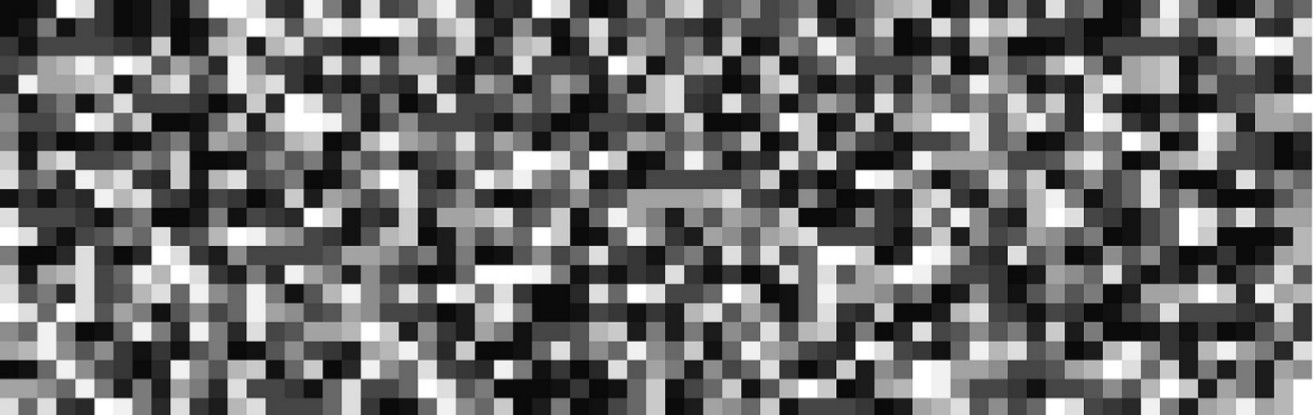
\includegraphics[width=\textwidth,height=0.7\textheight,keepaspectratio]{img/mineria/dnaimg_2}
		\label{img:mot2}
		\caption{Textures converted from the DNA sequences of Bacillus maritimus 16S ribosomal DNA.}
	\end{figure}
\end{frame}
%-------------------------------------------------------
%-------------------------------------------------------

%-------------------------------------------------------
%-------------------------------------------------------
\begin{frame}{FOS}{Histogram}
	\begin{figure}[]
		\centering
		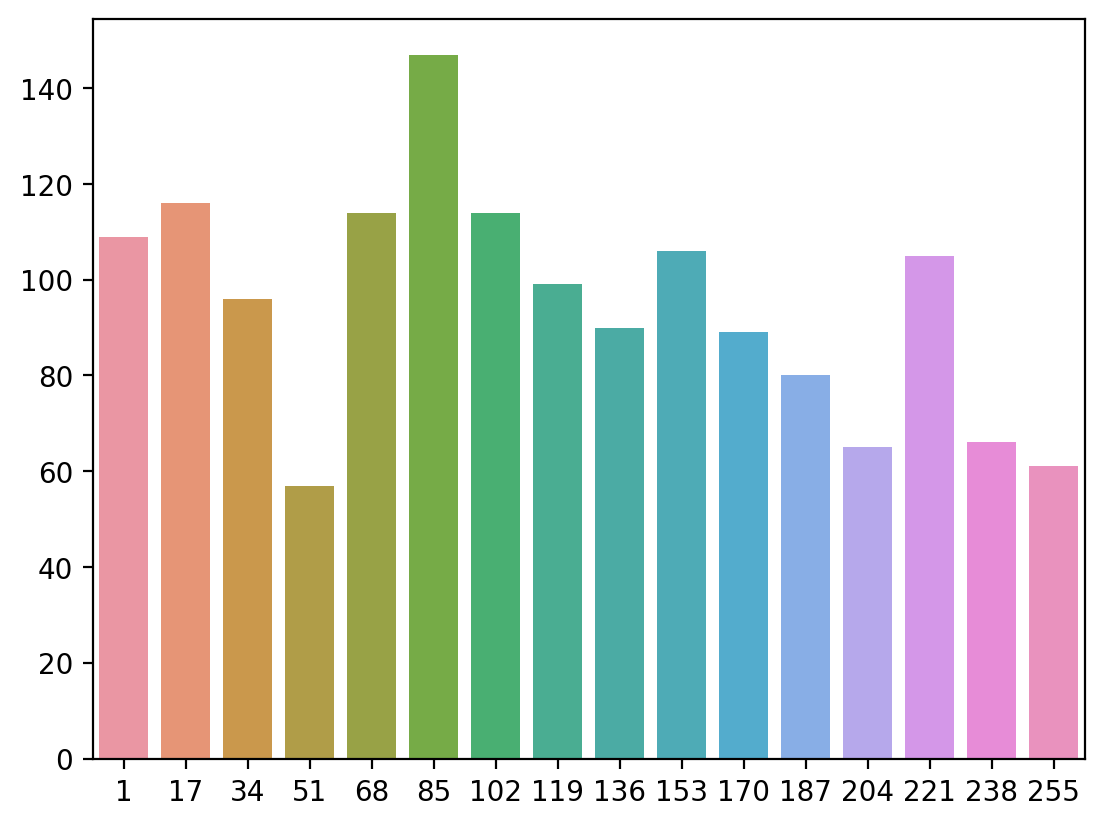
\includegraphics[width=0.6\textwidth,keepaspectratio]{img/mineria/histogram}
		\label{img:mot2}
		\caption{Histogram of Bacillus maritimus 16S ribosomal DNA. }
	\end{figure}
\end{frame}
%-------------------------------------------------------
%-------------------------------------------------------

%-------------------------------------------------------
%-------------------------------------------------------
\begin{frame}{FOS}{Features}
	\begin{block}{}
		From the histogram, the following features are compute:
		\begin{itemize}
			\item \textbf{\textit{Skewness}} $ = \sigma^{-3} \sum_{i=0}^{G-1} (i - \mu)^3 p(i)$
			\item \textbf{\textit{Kurtosis}} $ = \sigma^{-4} \sum_{i=0}^{G-1} (i - \mu)^4 p(i)-3$
			\item \textbf{\textit{Energy}} $ = \sum_{i=0}^{G-1} p(i)^2$
			\item \textbf{\textit{Entropy}} $ = -\sum_{i=0}^{G-1} p(i)lg(p(i))$
		\end{itemize}
	\end{block}
	
	\begin{block}{}
		Where: 
		\begin{itemize}	
			\item	$p(i) = h(i)/NM$ 
			\item	$h(i) =$ \textit{histogram} 
			\item	$N$ and $M$ \textit{are image's width and height.} 
			\item	$\mu = \sum_{i=0}^{G-1}ip(i)$
		\end{itemize}
	\end{block}
\end{frame}
%-------------------------------------------------------
%-------------------------------------------------------

%%%%%%%%%%%%%%%%%%%%%%%%%%%%%%%%%%%%%%%%%%%%%%%%%%%%%%%%%%%%%%%%%%%%%%%%%%%%%%%%%%%%%%%%%%%%%%%%%%%%%%%%%%%%%%%%
%%%%%%%%%%%%%%%%%%%%%%%%%%%%%%%%%%%%%%%%%%%%%%%%%%%%%%%%%%%%%%%%%%%%%%%%%%%%%%%%%%%%%%%%%%%%%%%%%%%%%%%%%%%%%%%%
\subsection{Gray Level Co-ocurrence Matrix (GLCM)} \label{section:glcm}
%%%%%%%%%%%%%%%%%%%%%%%%%%%%%%%%%%%%%%%%%%%%%%%%%%%%%%%%%%%%%%%%%%%%%%%%%%%%%%%%%%%%%%%%%%%%%%%%%%%%%%%%%%%%%%%%
%%%%%%%%%%%%%%%%%%%%%%%%%%%%%%%%%%%%%%%%%%%%%%%%%%%%%%%%%%%%%%%%%%%%%%%%%%%%%%%%%%%%%%%%%%%%%%%%%%%%%%%%%%%%%%%%


%-------------------------------------------------------
%-------------------------------------------------------
\begin{frame}{GLCM}{Mapping function}
	\begin{block}{}
		Each base in sequence $S = \{A, C, G, T\}$ is mapped to the numbers $S' = \{ 1, 2, 3, 4 \}$. Then we added to each value the base position. 
	\end{block}

	\begin{figure}[]
		\centering
		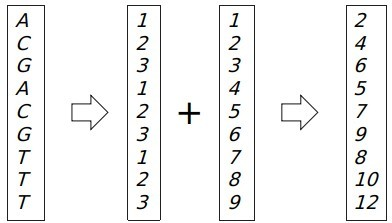
\includegraphics[width=0.6\textwidth,keepaspectratio]{img/mineria/vectordna}		
	\end{figure}

	\begin{block}{}
		Then, compute  gray-level co-occurrence matrix.
	\end{block}
\end{frame}
%-------------------------------------------------------
%-------------------------------------------------------

%-------------------------------------------------------
%-------------------------------------------------------
\begin{frame}{GLCM}{Mapping function}
	 \begin{figure}[h]
		\centering
		\begin{multicols}{2}
			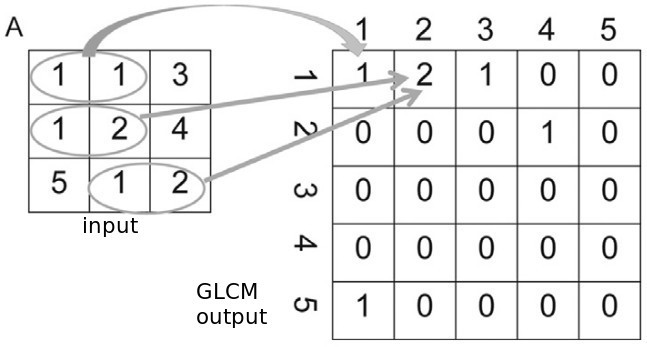
\includegraphics[width=0.45\textwidth,keepaspectratio]{img/mineria/glcm}\par 
			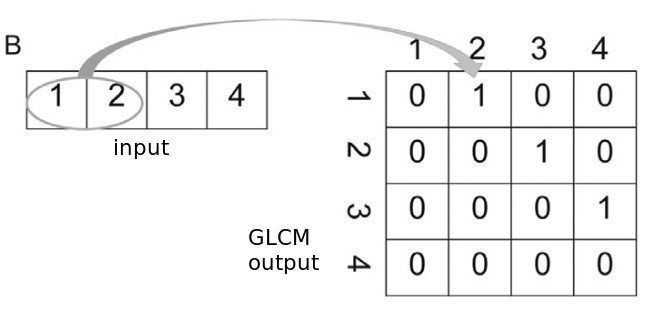
\includegraphics[width=0.45\textwidth,keepaspectratio]{img/mineria/glcm2}\par 
		\end{multicols}
		\caption{Examples of GLCM algorithm. Left: GLCM computed from a 2D matrix with intensities from 1 to 5.  Right: GLCM computed from a 1D vector with intensities from 1 to 4.}
		\label{img:glcm}
	\end{figure}
\end{frame}
%-------------------------------------------------------
%-------------------------------------------------------

%-------------------------------------------------------
%-------------------------------------------------------
\begin{frame}{GLCM}{Features}
	\begin{block}{}
		From the histogram, the following features are compute:
		\begin{itemize}
			\item \textbf{\textit{Entropy}} $ = -\sum_{i=1}^{L}\sum_{j=1}^{L} p(i, j)Ln(p(i,j))$
			\item \textbf{\textit{Contrast}} $  =  \sum_{i=1}^{L}\sum_{j=1}^{L} (i-j)^2 p(i, j)$
			\item \textbf{\textit{Energy}} $ =  \sum_{i=1}^{L}\sum_{j=1}^{L} p(i,j)^2$
			\item \textbf{\textit{Correlation}} $ =  \sum_{i=1}^{L}\sum_{j=1}^{L}  \frac{ (i - \mu_i)(j - \mu_i)p(i, j)  }{ \sigma_i \sigma_j }     $
			\item \textbf{\textit{Homogeneity}} $ =  \sum_{i=1}^{L}\sum_{j=1}^{L}  \frac{ p(i, j) }{ 1 + | i - j | }    $
		\end{itemize}
	\end{block}
	
	\begin{block}{}
		where, $p(i, j)$ is the GLCM matrix and $L$ is the maximun intensity value.
		
	\end{block}
\end{frame}
%-------------------------------------------------------
%-------------------------------------------------------



%%%%%%%%%%%%%%%%%%%%%%%%%%%%%%%%%%%%%%%%%%%%%%%%%%%%%%%%%%%%%%%%%%%%%%%%%%%%%%%%%%%%%%%%%%%%%%%%%%%%%%%%%%%%%%%%
%%%%%%%%%%%%%%%%%%%%%%%%%%%%%%%%%%%%%%%%%%%%%%%%%%%%%%%%%%%%%%%%%%%%%%%%%%%%%%%%%%%%%%%%%%%%%%%%%%%%%%%%%%%%%%%%
\subsection{Multi-resolution Local Binary Patterns (MLBP)}
%%%%%%%%%%%%%%%%%%%%%%%%%%%%%%%%%%%%%%%%%%%%%%%%%%%%%%%%%%%%%%%%%%%%%%%%%%%%%%%%%%%%%%%%%%%%%%%%%%%%%%%%%%%%%%%%
%%%%%%%%%%%%%%%%%%%%%%%%%%%%%%%%%%%%%%%%%%%%%%%%%%%%%%%%%%%%%%%%%%%%%%%%%%%%%%%%%%%%%%%%%%%%%%%%%%%%%%%%%%%%%%%%

%-------------------------------------------------------
%-------------------------------------------------------
\begin{frame}{MLBP}{Mapping function}
	\begin{table}[h]
		\centering
		\caption{Numeric representation for each base used by Kouchaki et al. \cite{kouchaki2019signal}.}
		\label{tab:chen_numeric}
		\setlength{\tabcolsep}{0.5em} % for the horizontal padding
		{\renewcommand{\arraystretch}{1}% for the vertical padding
			\begin{tabular}{lllll}
				\hline
				Base           	&  Integer & EIIP & Atomic  & Real \\ \hline
				A      			& 2 & 0.1260 & 70 & -1.5 \\ 
				T          	   	& -2 & 0.1335 & 78 & 1.5 \\ 
				C      			& -1 & 0.1340 & 58 & -0.5 \\ 
				G				& 2 & 0.0806 & 66 & 0.5 \\ \hline
			\end{tabular}
		}
	\end{table}
\end{frame}
%-------------------------------------------------------
%-------------------------------------------------------

%-------------------------------------------------------
%-------------------------------------------------------
\begin{frame}{MLBP}{LBP example}
	\begin{figure}[]
		\centering
		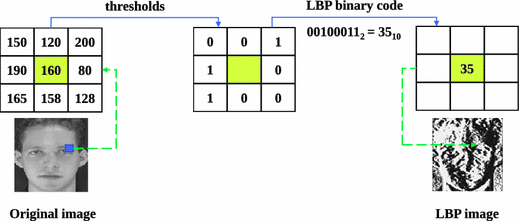
\includegraphics[width=\textwidth,keepaspectratio]{img/mineria/lbp.png}
		\label{img:mot2}
		\caption{Example of Local Binary Pattern algorithm. }
	\end{figure}
\end{frame}
%-------------------------------------------------------
%-------------------------------------------------------

%-------------------------------------------------------
%-------------------------------------------------------
\begin{frame}{MLBP}{Features}
	\begin{equation} \label{eq:mlbp}
	\begin{split}
	LBP(x(t)) =  \sum_{i=0}^{p/2 - 1} ( Sign ( x(t+i - p/2) - x(t) )2^i +  \\
	Sign( x(t+i+1) - x(t) )2^{i+p/2}  ),
	\end{split}
	\end{equation}		
	where $p$ in the number of neighbouring points and $Sign$ is:
	
	\begin{equation} \label{eq:sign}
	Sign(x) =   
	\begin{cases}
	0, & x < 0 \\
	1, & x \geq 0
	\end{cases}
	\end{equation}
	
	\begin{equation} \label{eq:kro}
	h_k = \sum_{ p/2 \leq i \leq N - p/2} \delta (LBP_p( x(i), k ) ),
	\end{equation}
\end{frame}
%-------------------------------------------------------
%-------------------------------------------------------




%%%%%%%%%%%%%%%%%%%%%%%%%%%%%%%%%%%%%%%%%%%%%%%%%%%%%%%%%%%%%%%%%%%%%%%%%%%%%%%%%%%%%%%%%%%%%%%%%%%%%%%%%%%%%%%%
%%%%%%%%%%%%%%%%%%%%%%%%%%%%%%%%%%%%%%%%%%%%%%%%%%%%%%%%%%%%%%%%%%%%%%%%%%%%%%%%%%%%%%%%%%%%%%%%%%%%%%%%%%%%%%%%
\section{Results}
%%%%%%%%%%%%%%%%%%%%%%%%%%%%%%%%%%%%%%%%%%%%%%%%%%%%%%%%%%%%%%%%%%%%%%%%%%%%%%%%%%%%%%%%%%%%%%%%%%%%%%%%%%%%%%%%
%%%%%%%%%%%%%%%%%%%%%%%%%%%%%%%%%%%%%%%%%%%%%%%%%%%%%%%%%%%%%%%%%%%%%%%%%%%%%%%%%%%%%%%%%%%%%%%%%%%%%%%%%%%%%%%%

%%%%%%%%%%%%%%%%%%%%%%%%%%%%%%%%%%%%%%%%%%%%%%%%%%%%%%%%%%%%%%%%%%%%%%%%%%%%%%%%%%%%%%%%%%%%%%%%%%%%%%%%%%%%%%%%
%%%%%%%%%%%%%%%%%%%%%%%%%%%%%%%%%%%%%%%%%%%%%%%%%%%%%%%%%%%%%%%%%%%%%%%%%%%%%%%%%%%%%%%%%%%%%%%%%%%%%%%%%%%%%%%%
\subsection{Datasets}
%%%%%%%%%%%%%%%%%%%%%%%%%%%%%%%%%%%%%%%%%%%%%%%%%%%%%%%%%%%%%%%%%%%%%%%%%%%%%%%%%%%%%%%%%%%%%%%%%%%%%%%%%%%%%%%%
%%%%%%%%%%%%%%%%%%%%%%%%%%%%%%%%%%%%%%%%%%%%%%%%%%%%%%%%%%%%%%%%%%%%%%%%%%%%%%%%%%%%%%%%%%%%%%%%%%%%%%%%%%%%%%%%

%-------------------------------------------------------
%-------------------------------------------------------
\begin{frame}{Datasets}
	\begin{table}[]
		\centering
		\caption{16S ribosomal DNA of 13 bacteria.}
		\label{tab:16sdb}
		\begin{tabular}{llll}
			\hline
			Species                         & Accesion Code & Length (bp) \\ \hline
			Bacillus       maritimus         & KP317497      & 1515        \\
			Bacillus       wakoensis         & NR\_040849    & 1524        \\
			Bacillus       australimaris     & NR\_148787    & 1513        \\
			Bacillus       xiamenensis       & NR\_148244    & 1513        \\
			Escherichia    coli              & J01859        & 1541        \\
			Streptococcus  himalayensis      & NR\_156072    & 1509        \\
			Streptococcus  halotolerans      & NR\_152063    & 1520        \\
			Streptococcus  tangierensis      & NR\_134818    & 1520        \\
			Streptococcus  cameli            & NR\_134817    & 1518        \\
			Thermus        amyloliquefaciens & NR\_136784    & 1514        \\
			Thermus        tengchongensis    & NR\_132306    & 1523        \\
			Thermus        thermophilus      & NR\_037066    & 1515        \\
			Thermus        filiformis        & NR\_117152    & 1514        \\ \hline
		\end{tabular} 
	\end{table}
\end{frame}
%-------------------------------------------------------
%-------------------------------------------------------

%-------------------------------------------------------
%-------------------------------------------------------
\begin{frame}{Datasets}
\begin{table}[]
	\centering
	\caption{NADH dehydrogenase subunit 4 genes of 12 species genome information from NCBI.}
	\label{tab:nadhdb}
	\begin{tabular}{lll}
		\hline
		Species             & Accesion Code & Length (bp) \\ \hline
		Macaca fascicularis & M22653        & 896         \\
		Macaca fuscata      & M22651        & 896         \\
		Macaca mulatta      & M22650        & 896         \\
		Macaca sylvanus     & M22654        & 896         \\
		Saimiri sciureus    & M22655        & 893         \\
		Chimpanzee          & V00672        & 896         \\
		Lemur catta         & M22657        & 895         \\
		Gorilla             & V00658        & 896         \\
		Hylobates           & V00659        & 896         \\
		Sumatran Orangutan  & V00675        & 895         \\
		Tarsius syrichta    & M22656        & 895         \\
		Human               & L00016        & 896        \\ \hline
	\end{tabular}
\end{table}
\end{frame}
%-------------------------------------------------------
%-------------------------------------------------------

%-------------------------------------------------------
%-------------------------------------------------------
\begin{frame}{Datasets}
\begin{table}[]
	\centering
	\caption{The mitochondrial genome detailed information of 18 eutherian mammals from
		NCBI database.}
	\label{tab:mitocondrialdb}
	\begin{tabular}{lll}
		\hline
		Species           & Accesion Code & Length (bp) \\ \hline
		Human             & V00662        & 16569       \\
		Pygmy chimpanzee  & D38116        & 16563       \\
		Common chimpanzee & D38113        & 16554       \\
		Gorilla           & D38114        & 16364       \\
		Orangutan         & D38115        & 16389       \\
		Gibbon            & X99256        & 16472       \\
		Baboon            & Y18001        & 16521       \\
		Horse             & X79547        & 16660       \\
		White rhinoceros  & Y07726        & 16832       \\
		Harbor seal       & X63726        & 16826       \\
		Gray seal         & X72004        & 16797       \\
		Cat               & U20753        & 17009       \\
		Fin whale         & X61145        & 16397       \\
		... & & \\
	\end{tabular}
\end{table}
\end{frame}
%-------------------------------------------------------
%-------------------------------------------------------



%-------------------------------------------------------
%-------------------------------------------------------
\begin{frame}{Mapping functions}
	
	\begin{table}[h]
		\centering
		\caption{Numeric representation for each base.}
		\label{tab:mapping function}
		\setlength{\tabcolsep}{0.5em} % for the horizontal padding
		{\renewcommand{\arraystretch}{1}% for the vertical padding
			\begin{tabular}{ccccccc}
				\hline
				Base           	&  MAP0 & MAP1 	& MAP2  & MAP3 & MAP4 & MAP5 \\ \hline
				A      			& FOS & GLCM	& 2 & 0.1260 & 70 & -1.5 \\ 
				T          	   	& FOS	& GLCM	& -2 & 0.1335 & 78 & 1.5 \\ 
				C      			& FOS	& GLCM	& -1 & 0.1340 & 58 & -0.5 \\ 
				G				& FOS	& GLCM	& 2 & 0.0806 & 66 & 0.5 \\ \hline
			\end{tabular}
		}
	\end{table}
\end{frame}
%-------------------------------------------------------
%-------------------------------------------------------


%%%%%%%%%%%%%%%%%%%%%%%%%%%%%%%%%%%%%%%%%%%%%%%%%%%%%%%%%%%%%%%%%%%%%%%%%%%%%%%%%%%%%%%%%%%%%%%%%%%%%%%%%%%%%%%%
%%%%%%%%%%%%%%%%%%%%%%%%%%%%%%%%%%%%%%%%%%%%%%%%%%%%%%%%%%%%%%%%%%%%%%%%%%%%%%%%%%%%%%%%%%%%%%%%%%%%%%%%%%%%%%%%
\subsection{Comparison of FOS, GLCM, LBP and MLBP}
%%%%%%%%%%%%%%%%%%%%%%%%%%%%%%%%%%%%%%%%%%%%%%%%%%%%%%%%%%%%%%%%%%%%%%%%%%%%%%%%%%%%%%%%%%%%%%%%%%%%%%%%%%%%%%%%
%%%%%%%%%%%%%%%%%%%%%%%%%%%%%%%%%%%%%%%%%%%%%%%%%%%%%%%%%%%%%%%%%%%%%%%%%%%%%%%%%%%%%%%%%%%%%%%%%%%%%%%%%%%%%%%%

%-------------------------------------------------------
%-------------------------------------------------------
\begin{frame}{Results}{Comparison in 16S ribosomal DNA dataset}
\begin{figure}[]
	\centering
	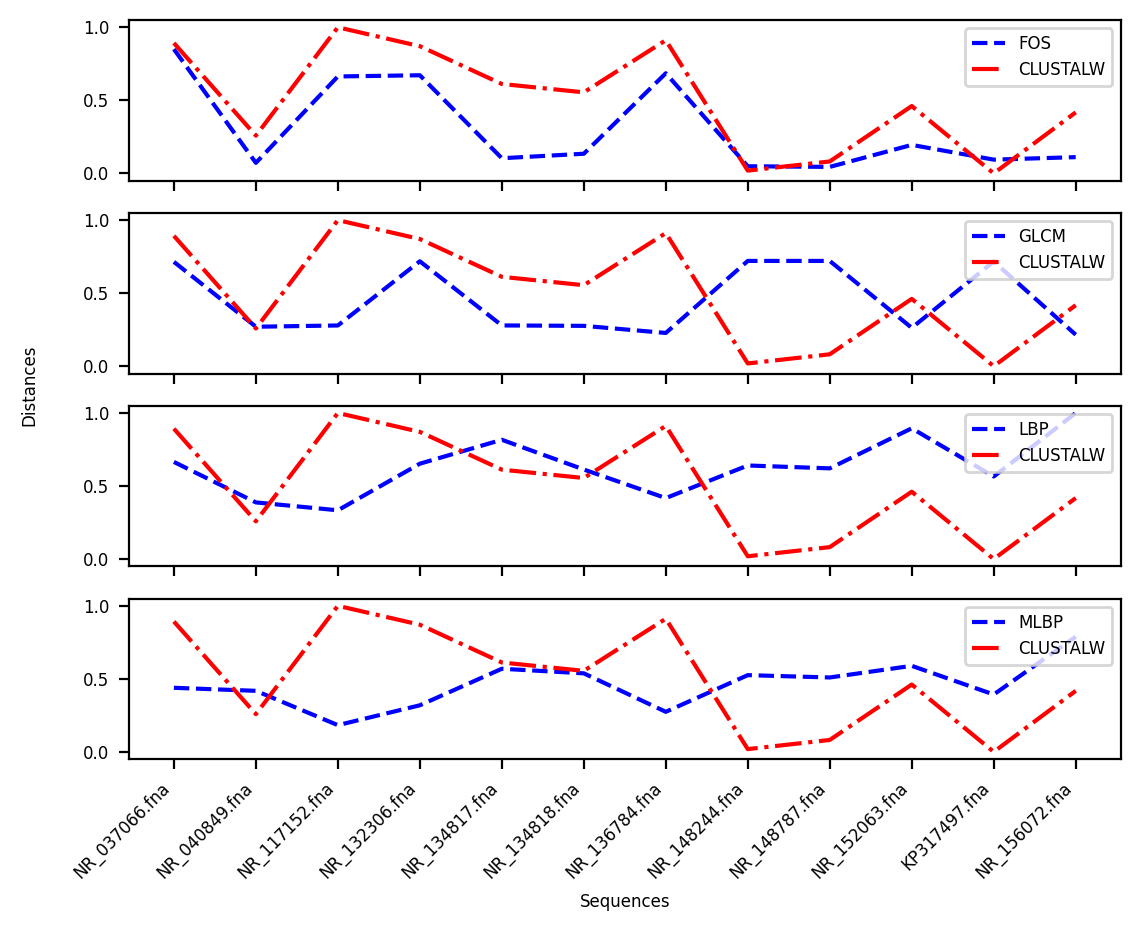
\includegraphics[width=0.7\textwidth,keepaspectratio]{img/mineria/db1}
	\caption{Euclidean distance of Escherichia coli against the rest sequences in 16S ribosomal DNA dataset. We used MEGA. FOS, GLCM, LBP and MLBP.}
	\label{img:comp1}
\end{figure}
\end{frame}
%-------------------------------------------------------
%-------------------------------------------------------

%-------------------------------------------------------
%-------------------------------------------------------
\begin{frame}{Results}{Comparison in NADH  dataset}
	\begin{figure}[hbt!]
		\centering
		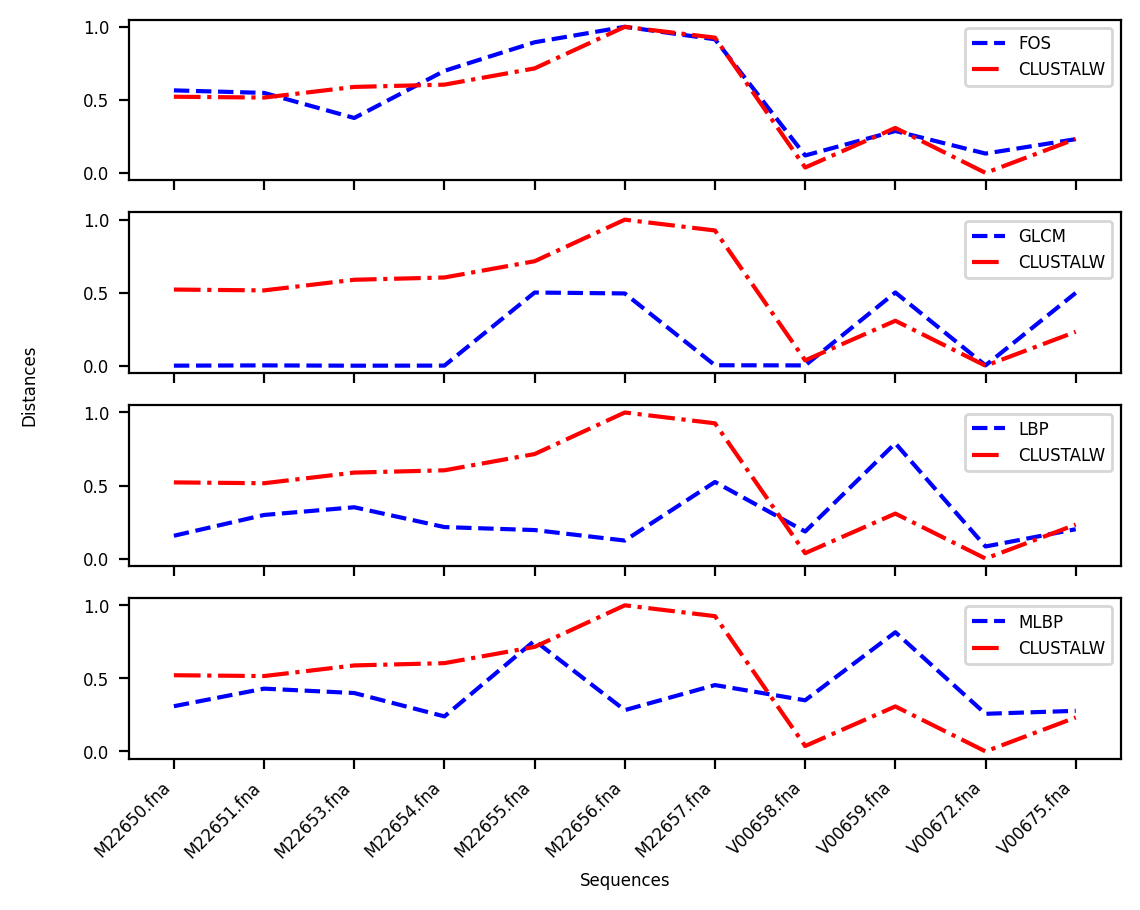
\includegraphics[width=0.7\textwidth,keepaspectratio]{img/mineria/db2}
		\caption{Euclidean distance of Human against the rest sequences in NADH dehydrogenase protein dataset. We used MEGA. FOS, GLCM, LBP and MLBP.}
		\label{img:comp2}
	\end{figure}
\end{frame}
%-------------------------------------------------------
%-------------------------------------------------------

%-------------------------------------------------------
%-------------------------------------------------------
\begin{frame}{Results}{Comparison in the mitochondrial dataset}
\begin{figure}[hbt!]
	\centering
	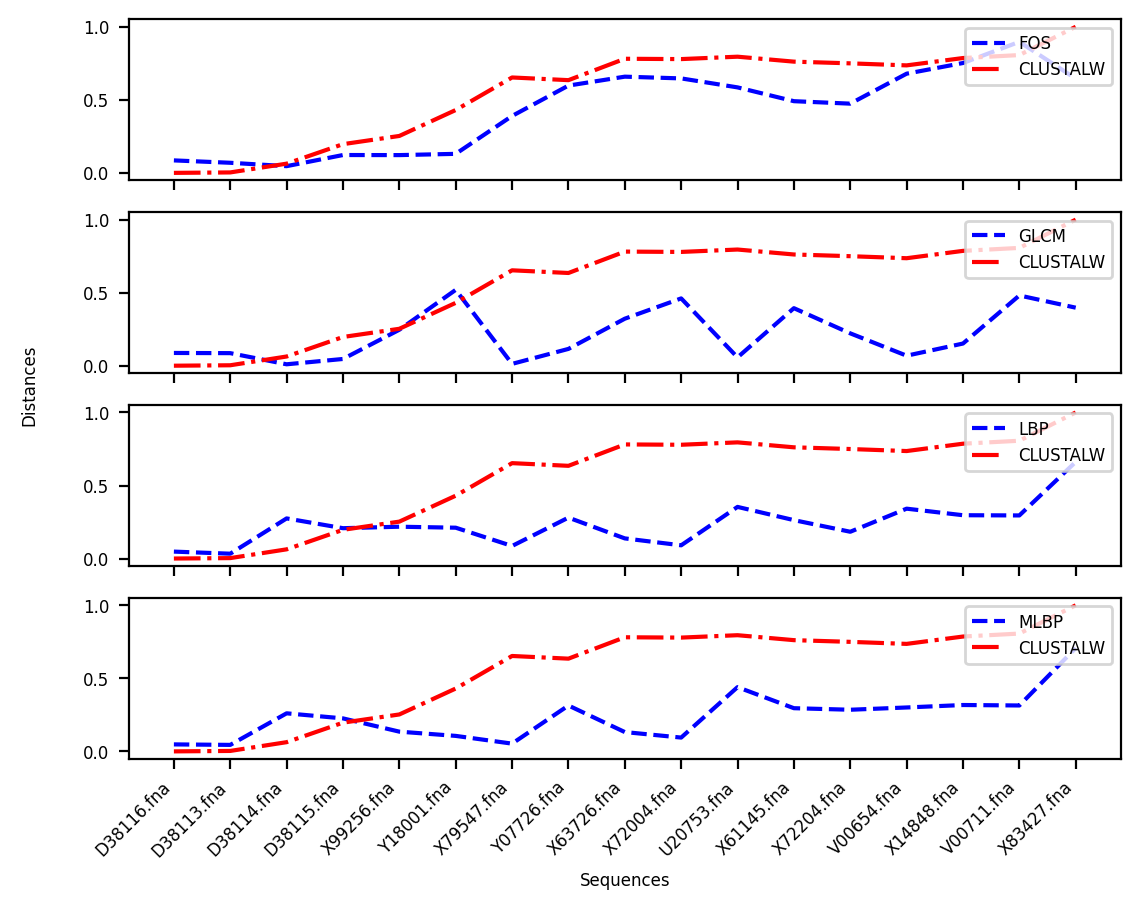
\includegraphics[width=0.7\textwidth,keepaspectratio]{img/mineria/db3}
	\caption{Euclidean distance of Human against the rest sequences in the mitochondrial genome dataset. We used MEGA. FOS, GLCM, LBP and MLBP.}
	\label{img:comp3}
\end{figure}
\end{frame}
%-------------------------------------------------------
%-------------------------------------------------------

%%%%%%%%%%%%%%%%%%%%%%%%%%%%%%%%%%%%%%%%%%%%%%%%%%%%%%%%%%%%%%%%%%%%%%%%%%%%%%%%%%%%%%%%%%%%%%%%%%%%%%%%%%%%%%%%
%%%%%%%%%%%%%%%%%%%%%%%%%%%%%%%%%%%%%%%%%%%%%%%%%%%%%%%%%%%%%%%%%%%%%%%%%%%%%%%%%%%%%%%%%%%%%%%%%%%%%%%%%%%%%%%%
\subsection{Comparison of mapping functions}
%%%%%%%%%%%%%%%%%%%%%%%%%%%%%%%%%%%%%%%%%%%%%%%%%%%%%%%%%%%%%%%%%%%%%%%%%%%%%%%%%%%%%%%%%%%%%%%%%%%%%%%%%%%%%%%%
%%%%%%%%%%%%%%%%%%%%%%%%%%%%%%%%%%%%%%%%%%%%%%%%%%%%%%%%%%%%%%%%%%%%%%%%%%%%%%%%%%%%%%%%%%%%%%%%%%%%%%%%%%%%%%%%


%-------------------------------------------------------
%-------------------------------------------------------
\begin{frame}{Results}{Comparison of the six mapping functions using FOS algorithm}
	\begin{figure}[]
		\centering
		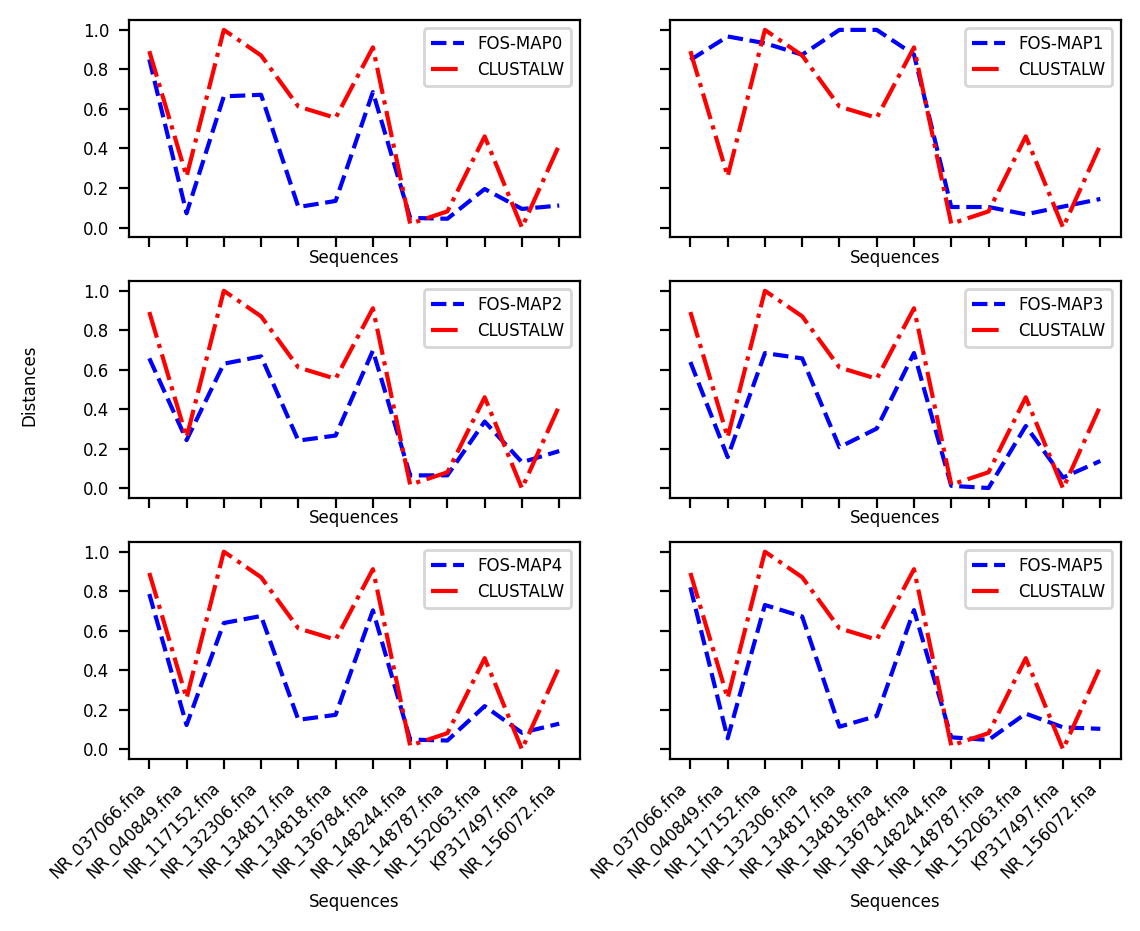
\includegraphics[width=0.7\textwidth,keepaspectratio]{img/mineria/db1_fos}
		\caption{Comparison of the 6 mapping functions using FOS algorithm over the 16S ribosomal DNA dataset.}
		\label{img:comp3}
	\end{figure}
\end{frame}
%-------------------------------------------------------
%-------------------------------------------------------

%-------------------------------------------------------
%-------------------------------------------------------
\begin{frame}{Results}{Comparison of MAP1 mapping function}
	\begin{figure}[]
		\centering
		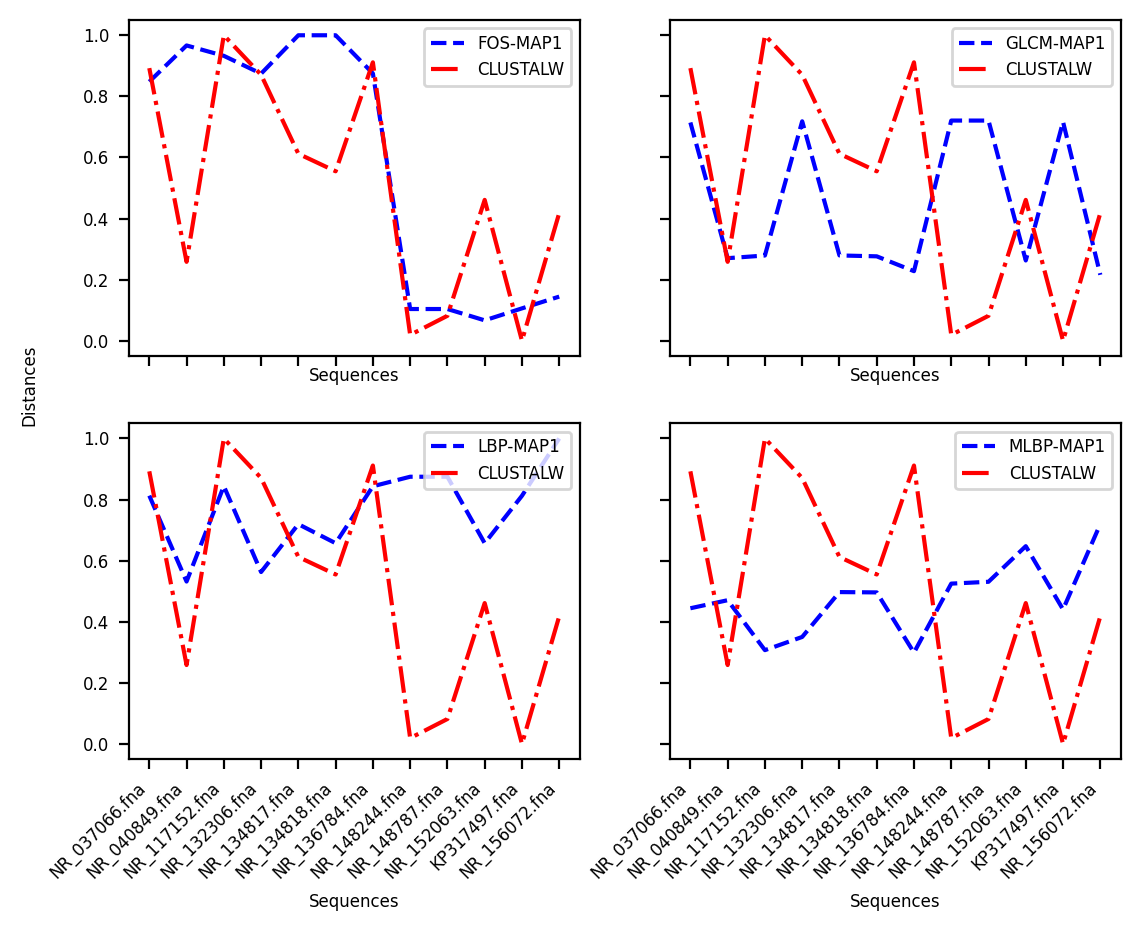
\includegraphics[width=0.7\textwidth,keepaspectratio]{img/mineria/db1_1map}
		\caption{Comparison of MAP1 mapping function over the 16S ribosomal DNA dataset.}
		\label{img:comp3}
	\end{figure}
\end{frame}
%-------------------------------------------------------
%-------------------------------------------------------

%-------------------------------------------------------
%-------------------------------------------------------
\begin{frame}{Results}{Comparison of the six mapping functions using GLCM algorithm}
	\begin{figure}[]
		\centering
		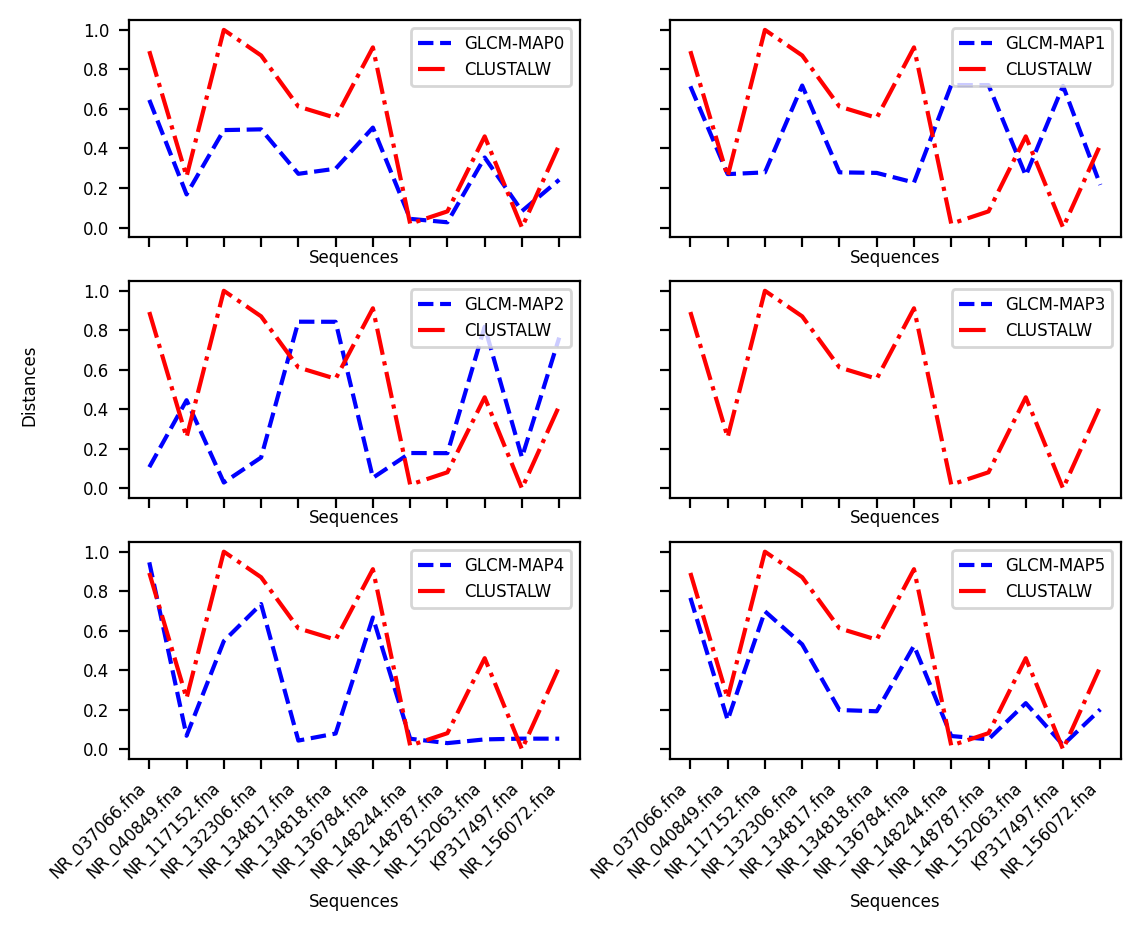
\includegraphics[width=0.7\textwidth,keepaspectratio]{img/mineria/db1_glcm}
		\caption{Comparison of the 6 mapping functions using GLCM algorithm over the 16S ribosomal DNA dataset.}
		\label{img:comp3}
	\end{figure}
\end{frame}
%-------------------------------------------------------
%-------------------------------------------------------

%%%%%%%%%%%%%%%%%%%%%%%%%%%%%%%%%%%%%%%%%%%%%%%%%%%%%%%%%%%%%%%%%%%%%%%%%%%%%%%%%
%DISCUCION
%%%%%%%%%%%%%%%%%%%%%%%%%%%%%%%%%%%%%%%%%%%%%%%%%%%%%%%%%%%%%%%%%%%%%%%%%%%%%%%%%

%-------------------------------------------------------
%-------------------------------------------------------
\begin{frame}{Results}{Discussion: Problem with MAP1 function}
	MAP1 function, proposed by Chen at el. \cite{chen2018use}.
	
	
	
			\begin{figure}[]
				\centering
				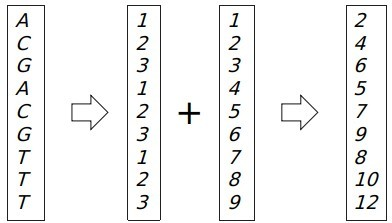
\includegraphics[width=0.4\textwidth,keepaspectratio]{img/mineria/vectordna}		
			\end{figure}
		
	

	\begin{block}{}
	The resultant vector have disperse values and it depends strongly from the sequence's length
	\end{block}
\end{frame}
%-------------------------------------------------------
%-------------------------------------------------------

%-------------------------------------------------------
%-------------------------------------------------------
\begin{frame}{Results}{Comparison of the six mapping functions using LBP algorithm}
	\begin{figure}[]
		\centering
		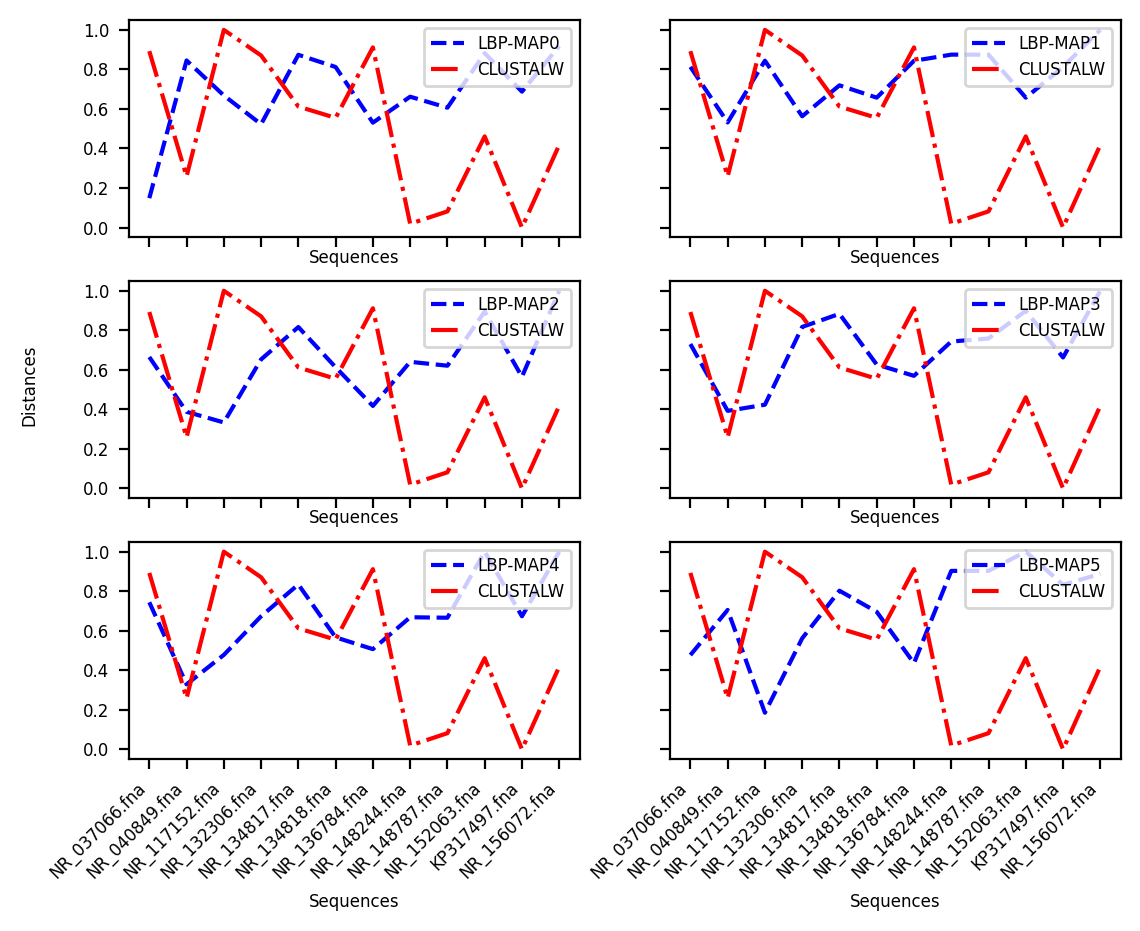
\includegraphics[width=0.7\textwidth,keepaspectratio]{img/mineria/db1_lbp}
		\caption{Comparison of the 6 mapping functions using the LBP algorithm over the 16S ribosomal DNA dataset.}
		\label{img:comp3}
	\end{figure}
\end{frame}
%-------------------------------------------------------
%-------------------------------------------------------

%-------------------------------------------------------
%-------------------------------------------------------
\begin{frame}{Results}{Comparison of the six mapping functions using MLBP algorithm}
	\begin{figure}[]
		\centering
		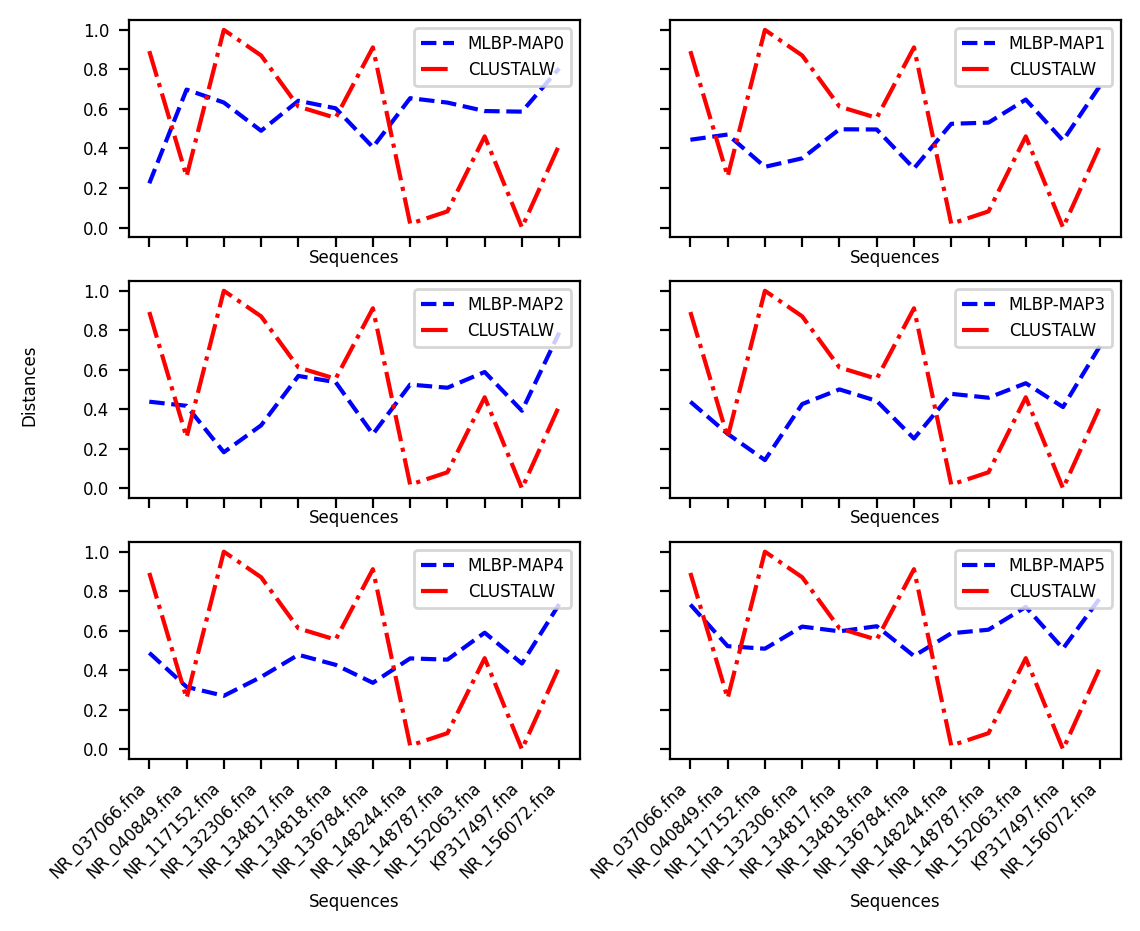
\includegraphics[width=0.7\textwidth,keepaspectratio]{img/mineria/db1_mlbp}
		\caption{Comparison of the 6 mapping functions using the MLBP algorithm over the 16S ribosomal DNA dataset.}
		\label{img:comp3}
	\end{figure}
\end{frame}
%-------------------------------------------------------
%-------------------------------------------------------


%-------------------------------------------------------
%-------------------------------------------------------
\begin{frame}{Results}{Square error of mapping functions and algorithms over the 16S ribosomal DNA dataset}
\begin{table}[hbt!]
	\centering
	\caption{Square error of all mapping functions and the four algorithms over the 16S ribosomal DNA dataset.}
	\label{tab:comparison_score_db1}
	\setlength{\tabcolsep}{0.5em} % for the horizontal padding
	{\renewcommand{\arraystretch}{1}% for the vertical padding
		\begin{tabular}{ccccc}
			\hline
			Mapping function    & FOS  & GLCM & LBP & MLBP \\ \hline
			MAP0 				& 0.07093 & 0.07214 & 0.2498 & 0.1997  \\
			MAP1 				& 0.09229 & 0.22709 & 0.2187 & 0.1805  \\
			MAP2 				& \textbf{0.04875} & 0.27343 & 0.1977 & 0.1965  \\
			MAP3 				& 0.05038 & 		 & 0.2106 & 0.1848  \\
			MAP4 				& 0.06267 & 0.09814 & 0.1997 & 0.1630  \\
			MAP5 				& 0.06592 & 0.06572 & 0.3395 & 0.1369  \\ \hline
		\end{tabular}
	}
\end{table}
\end{frame}
%-------------------------------------------------------
%-------------------------------------------------------

%-------------------------------------------------------
%-------------------------------------------------------
\begin{frame}{Results}{Square error of mapping functions and algorithms over the NADH dataset}
\begin{table}[hbt!]
	\centering
	\caption{Square error of all mapping functions and the four algorithms over the NADH dataset.}
	\label{tab:comparison_score_db2}
	\setlength{\tabcolsep}{0.5em} % for the horizontal padding
	{\renewcommand{\arraystretch}{1}% for the vertical padding
		\begin{tabular}{ccccc}
			\hline
			Mapping function    & FOS  		& GLCM & LBP & MLBP \\ \hline
			MAP0 				&	\textbf{0.0103} &	0.0345 &	0.0406 	& 0.0711 
			\\
			MAP1 				& 	0.1795 &	0.2279 &	0.2029 &	0.0895 
			\\
			MAP2 				&	0.0126 &	0.0307 &	0.1682 &	0.1258 
			\\
			MAP3 				&	0.1642 &			& 	0.1310 &	0.1022 
			\\
			MAP4 				&	0.0297 &	0.0784 &	0.1410 &	0.0630 
			\\
			MAP5 				&	0.0865 &	0.0345 &	0.0792 &	0.0452 \\ \hline
		\end{tabular}
	}
\end{table}
\end{frame}
%-------------------------------------------------------
%-------------------------------------------------------

%-------------------------------------------------------
%-------------------------------------------------------
\begin{frame}{Results}{Square error of mapping functions and algorithms over the mitochondrial genome dataset}
\begin{table}[hbt!]
	\centering
	\caption{Square error of all mapping functions and the four algorithms over the mitochondrial genome dataset.}
	\label{tab:comparison_score_db3}
	\setlength{\tabcolsep}{0.5em} % for the horizontal padding
	{\renewcommand{\arraystretch}{1}% for the vertical padding
		\begin{tabular}{ccccc}
			\hline
			Mapping function    & FOS  		& GLCM & LBP & MLBP \\ \hline
			MAP0 &	\textbf{0.0329} &	0.0569 &	0.1693 &	0.1254 
			\\
			MAP1 &	0.2439 &	0.1951 &	0.1294 &	0.1465 
			\\
			MAP2 &	0.0417 &	0.1567 &	0.1746 &	0.1654 
			\\
			MAP3 &	0.1811 & &		0.0768 &	0.1094 
			\\
			MAP4 &	0.0570 &	0.0731 &	0.1765 &	0.1724 
			\\
			MAP5 &	0.1255 &	0.0851 &	0.1622 & 	0.1575 
			\\ \hline
			
		\end{tabular}
	}
\end{table}
\end{frame}
%-------------------------------------------------------
%-------------------------------------------------------

%-------------------------------------------------------
%-------------------------------------------------------
\begin{frame}{Results}{Discussion: Best mapping function}
	MAP0 function and histogram proposed by Deliba et al. \cite{delibacs2020dna} is very similar to k-mer frecuencies.  \cite{karlin1994comparisons, campbell1999genome, shedlock2007phylogenomics, wu2001statistical, sims2009alignment, sims2011whole, wu2005optimal, dai2008markov, haubold2014alignment, karamichalis2015investigation, vinga2003alignment}
	
	
	\begin{columns}
		\begin{column}{0.48\textwidth}
			\begin{figure}[]
				\centering
				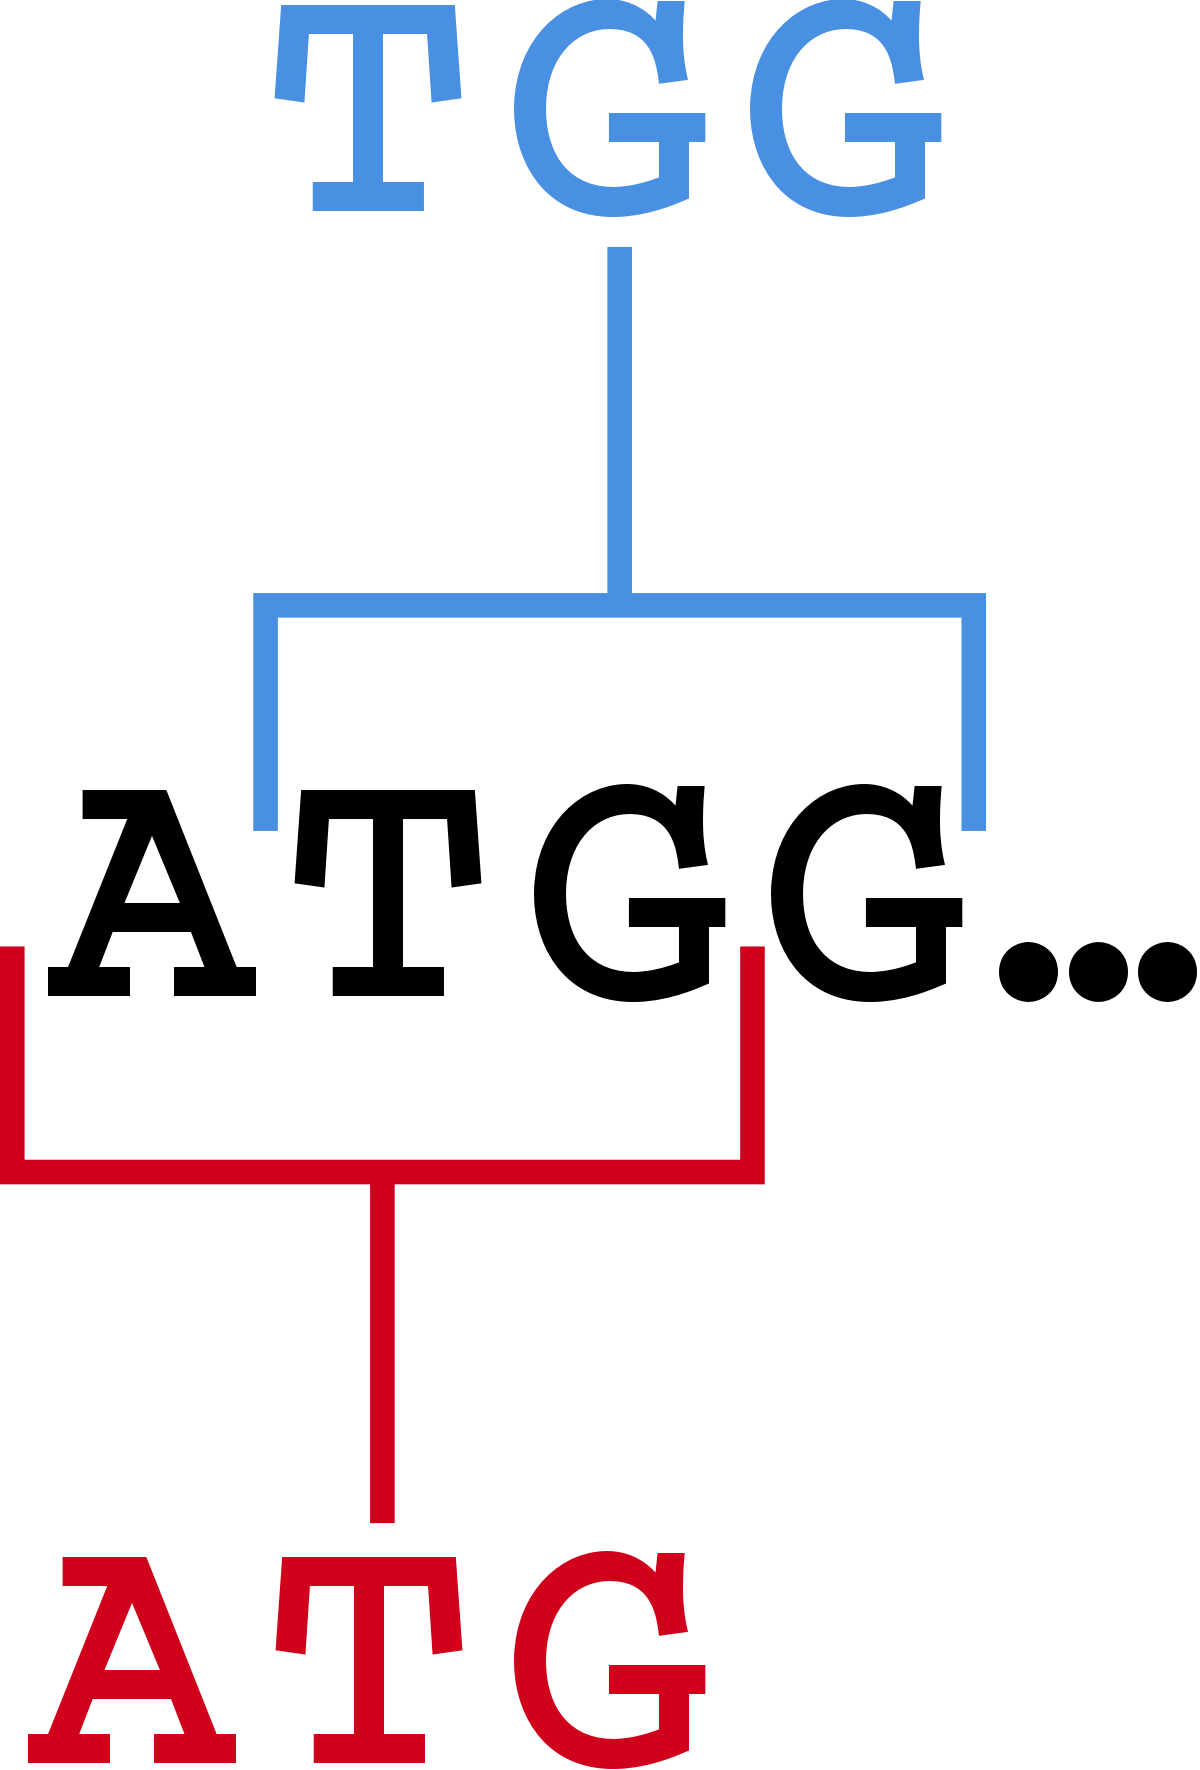
\includegraphics[width=0.4\textwidth,keepaspectratio]{img/mineria/kmer}		
			\end{figure}
		\end{column}
		\begin{column}{0.48\textwidth}
			\begin{figure}[]
				\centering
				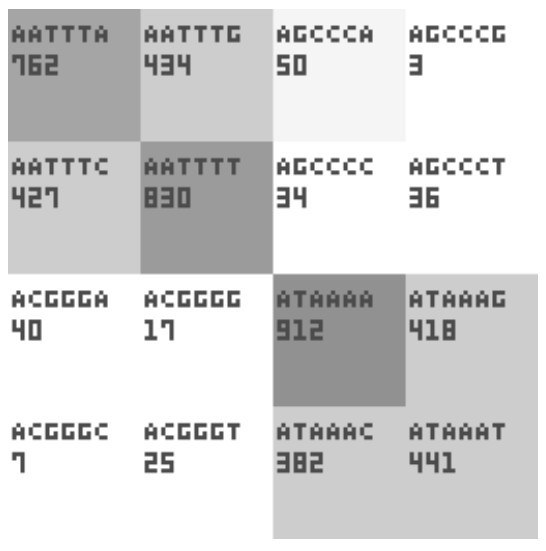
\includegraphics[width=0.6\textwidth,keepaspectratio]{img/mineria/cgr3}		
			\end{figure}
		\end{column}
	\end{columns}
	
	\begin{block}{}
		LBP and MLBP reflects the correlation among pixels within a local area, but the main infomration in DNA sequences is no related to correlations of neighbors bases.
	\end{block}

	

\end{frame}
%-------------------------------------------------------
%-------------------------------------------------------




%%%%%%%%%%%%%%%%%%%%%%%%%%%%%%%%%%%%%%%%%%%%%%%%%%%%%%%%%%%%%%%%%%%%%%%%%%%%%%%%%%%%%%%%%%%%%%%%%%%%%%%%%%%%%%%%
%%%%%%%%%%%%%%%%%%%%%%%%%%%%%%%%%%%%%%%%%%%%%%%%%%%%%%%%%%%%%%%%%%%%%%%%%%%%%%%%%%%%%%%%%%%%%%%%%%%%%%%%%%%%%%%%
\section{Conclusions}
%%%%%%%%%%%%%%%%%%%%%%%%%%%%%%%%%%%%%%%%%%%%%%%%%%%%%%%%%%%%%%%%%%%%%%%%%%%%%%%%%%%%%%%%%%%%%%%%%%%%%%%%%%%%%%%%
%%%%%%%%%%%%%%%%%%%%%%%%%%%%%%%%%%%%%%%%%%%%%%%%%%%%%%%%%%%%%%%%%%%%%%%%%%%%%%%%%%%%%%%%%%%%%%%%%%%%%%%%%%%%%%%%
%-------------------------------------------------------
%-------------------------------------------------------
\begin{frame}{Conclusions}{}
	\begin{itemize}
		\item We compared FOS, GLCM, LBP, and MLBP with six mapping functions. We also, compare the phylogenetic trees with Robinson Fould algorithm and Phylo.io. \pause
		\item FOS got the best results. Moreover, MAP1 was the worst mapping function and MAP0 was the best because of its similarity to k-mer method. \pause
		\item LBP and MLBP are not suitable for sequence similarity because they consider the correlation between neighbors. \pause
		\item Furthermore, FOS's tree is the most similar to MEGA's tree for the NADH dehydrogenase and the mitochondrial genomes datasets.
	\end{itemize}
\end{frame}
%-------------------------------------------------------
%-------------------------------------------------------

%-------------------------------------------------------
%-------------------------------------------------------
%\begin{frame}{Proposal}{Visualization}

%	\begin{figure}[]
%		\centering
%		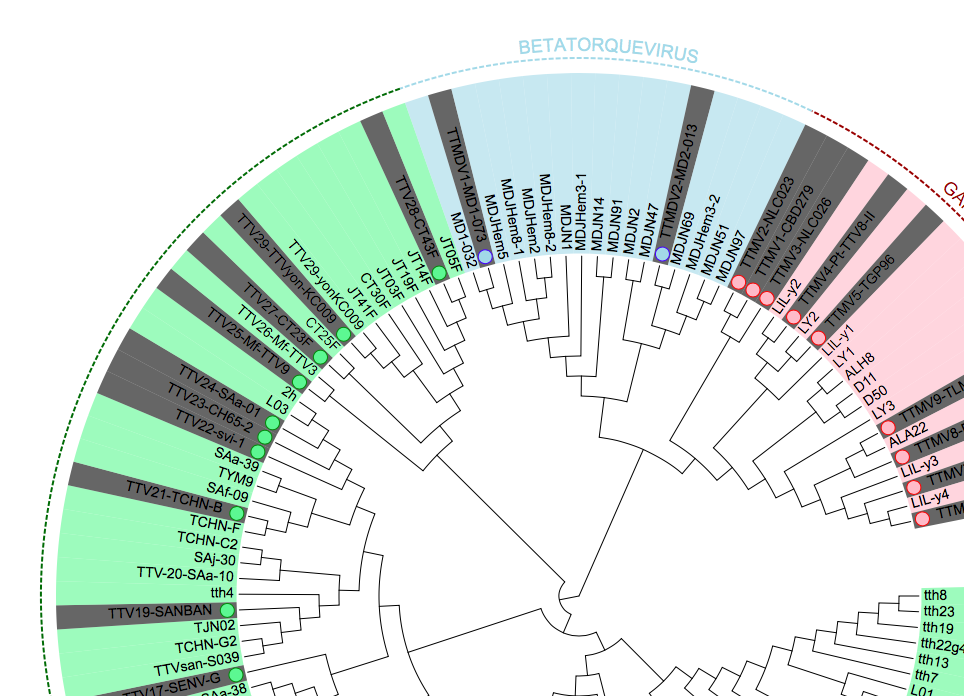
\includegraphics[width=0.7\textwidth,keepaspectratio]{img/mineria/tree2}
%		\label{img:mot2}
%		%\caption{Phylogenetic tree generated by the proposed method. Source: \cite{delibacs2020dna} }
%	\end{figure}
%\end{frame}
%-------------------------------------------------------
%-------------------------------------------------------




%-------------------------------------------------------
%-------------------------------------------------------
\begin{frame}[allowframebreaks]
\frametitle{References}
%\bibliographystyle{amsalpha}
\bibliographystyle{IEEEtran}
\bibliography{bibliography.bib}
\end{frame}
%-------------------------------------------------------
%-------------------------------------------------------


%-------------------------------------------------------
%-------------------------------------------------------
\if\mycmd1 % MY THEME
	\begin{frame}[plain,noframenumbering]
		%\finalpage{Thank you}
		\begin{figure}[]
			\centering
			
\includegraphics[width=\textwidth,height=0.7\textheight,keepaspectratio]{img/question.png}
			%\label{img:mot2}
			%\caption{Image example in 2 gray levels.}
		\end{figure}
	\end{frame}
	
\else % CS THEME
\begin{frame}{Questions?}
	\begin{figure}[]
		\centering
		
\includegraphics[width=\textwidth,height=0.7\textheight,keepaspectratio]{img/question.png}
		%\label{img:mot2}
		%\caption{Image example in 2 gray levels.}
	\end{figure}
	
\end{frame}
\fi
%-------------------------------------------------------
%-------------------------------------------------------
	
	
\end{document}